\part{平面几何练习题}
\section{导角法}

% \begin{exercise}
% 在四边形 $WXYZ$ 中,对角线相互垂直,已知 $\angle WZX = 30^\circ$,$\angle XWY = 40^\circ$,$\angle WYZ = 50^\circ$。
% (a) 求 $\angle WZY$;
% (b) 求 $\angle WXY$。
% \end{exercise}
% \begin{figure}[H]
%     \centering
%     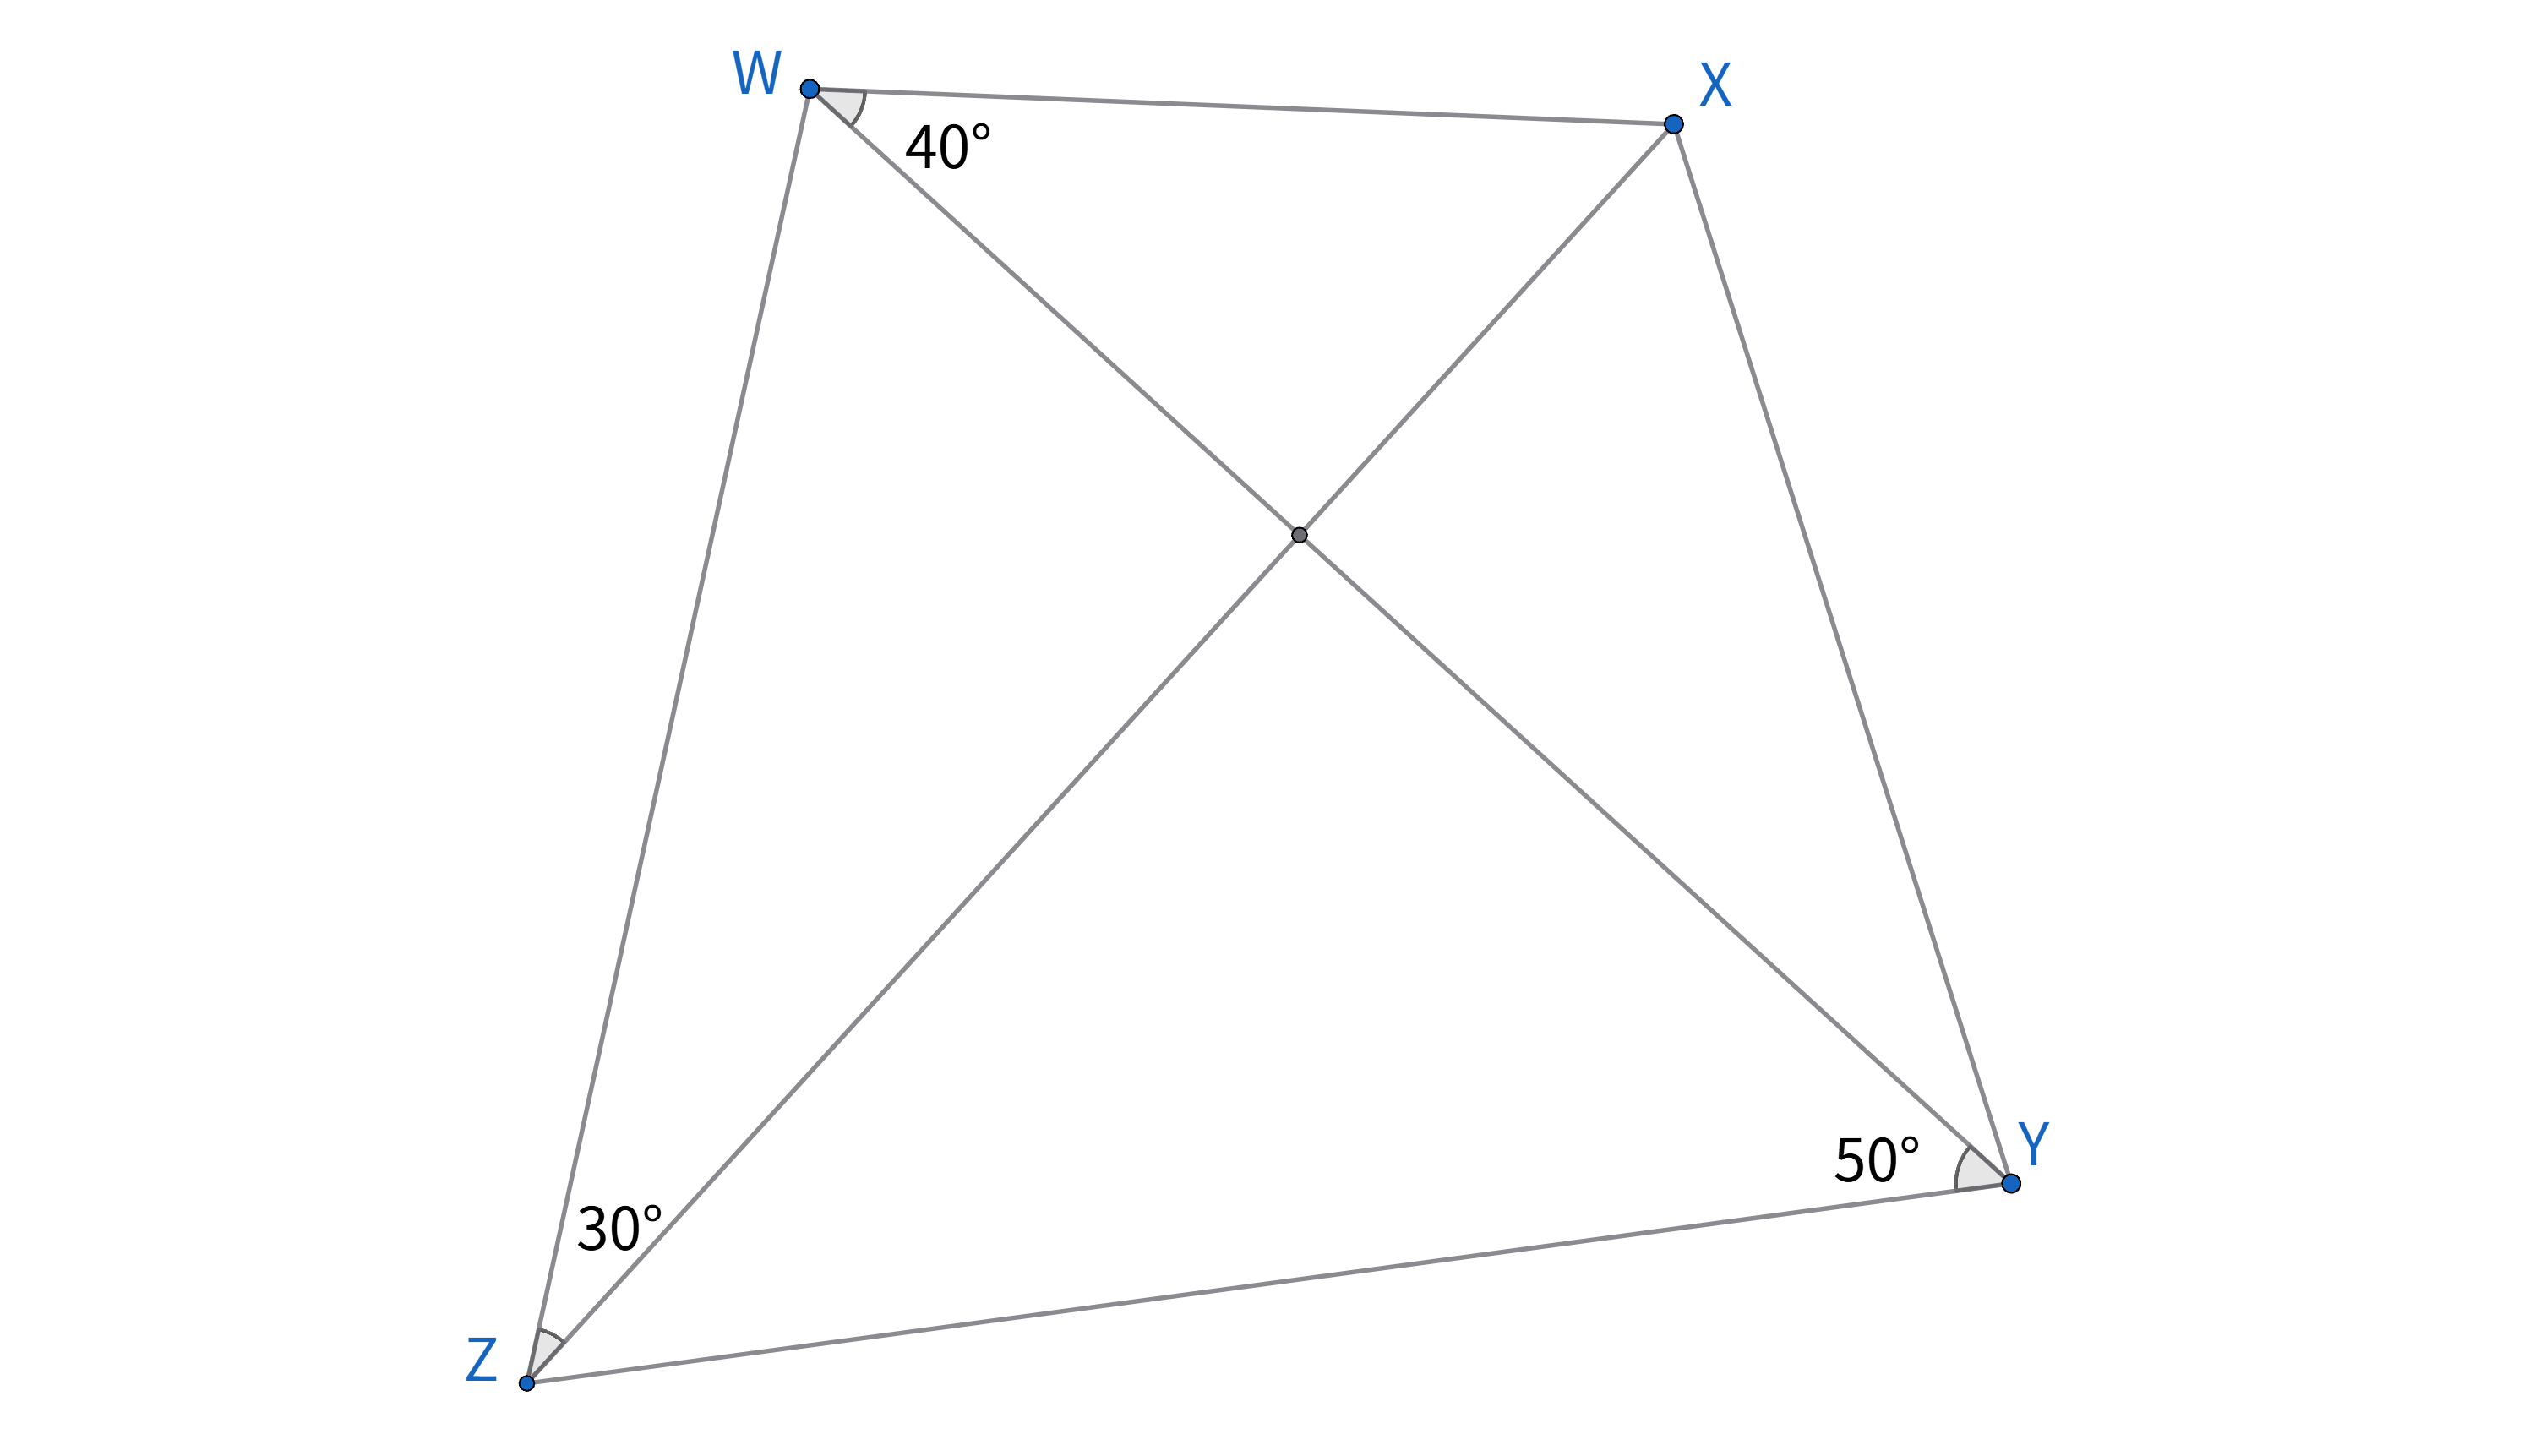
\includegraphics[width=0.7\linewidth]{figures/exercises/001.png}
% \end{figure}

% \begin{exercise}
% 设 $ABCDE$ 是一个凸五边形,其中 $BCDE$ 是正方形,中心为 $O$,$\angle A = 90^\circ$。证明:$AO$ 平分 $\angle BAE$。
% \end{exercise}
% \begin{figure}[H]
%     \centering
%     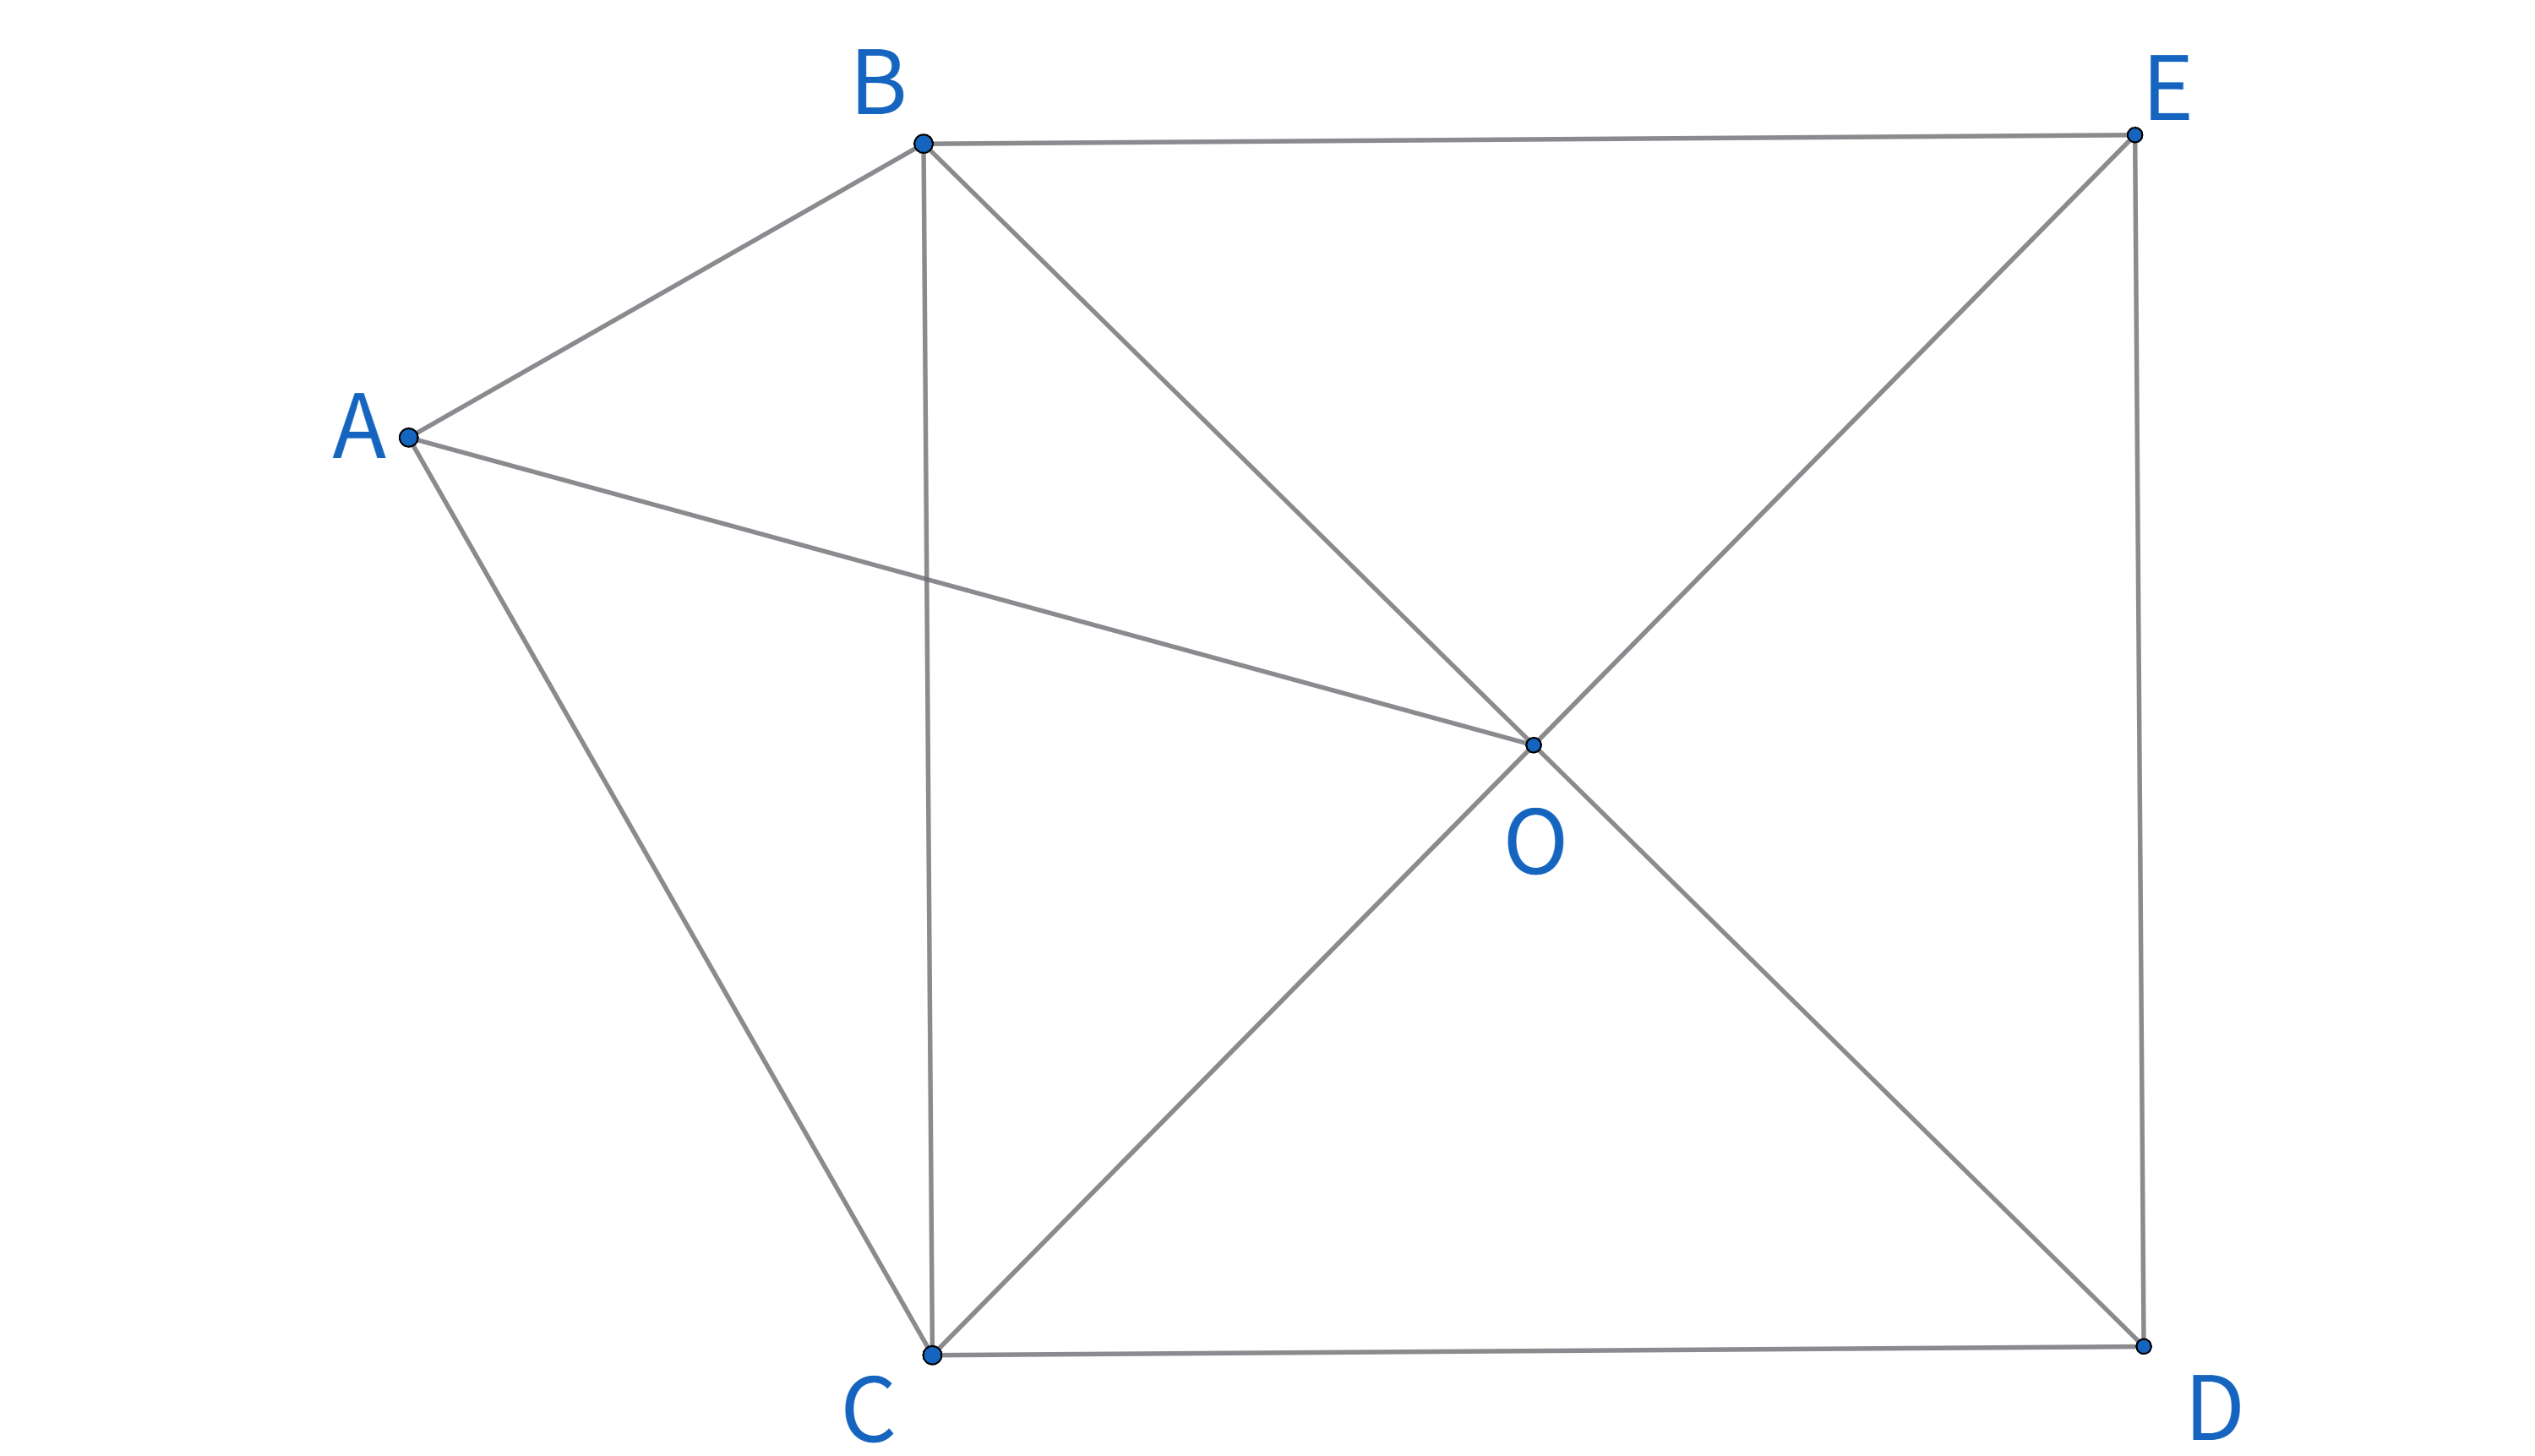
\includegraphics[width=0.7\linewidth]{figures/exercises/002.png}
% \end{figure}

\newpage 
\begin{exercise}
(BAMO 1999/2) 设 $O = (0, 0)$,$A = (0, a)$,$B = (0, b)$,其中实数 $0 < a < b$。设 $\Gamma$ 是直径为 ${AB}$ 的圆,$P$ 是 $\Gamma$ 上另一点。直线 $PA$ 与 $x$ 轴交于点 $Q$。证明:$\angle BQP = \angle BOP$。
\end{exercise}
\begin{figure}[H]
    \centering
    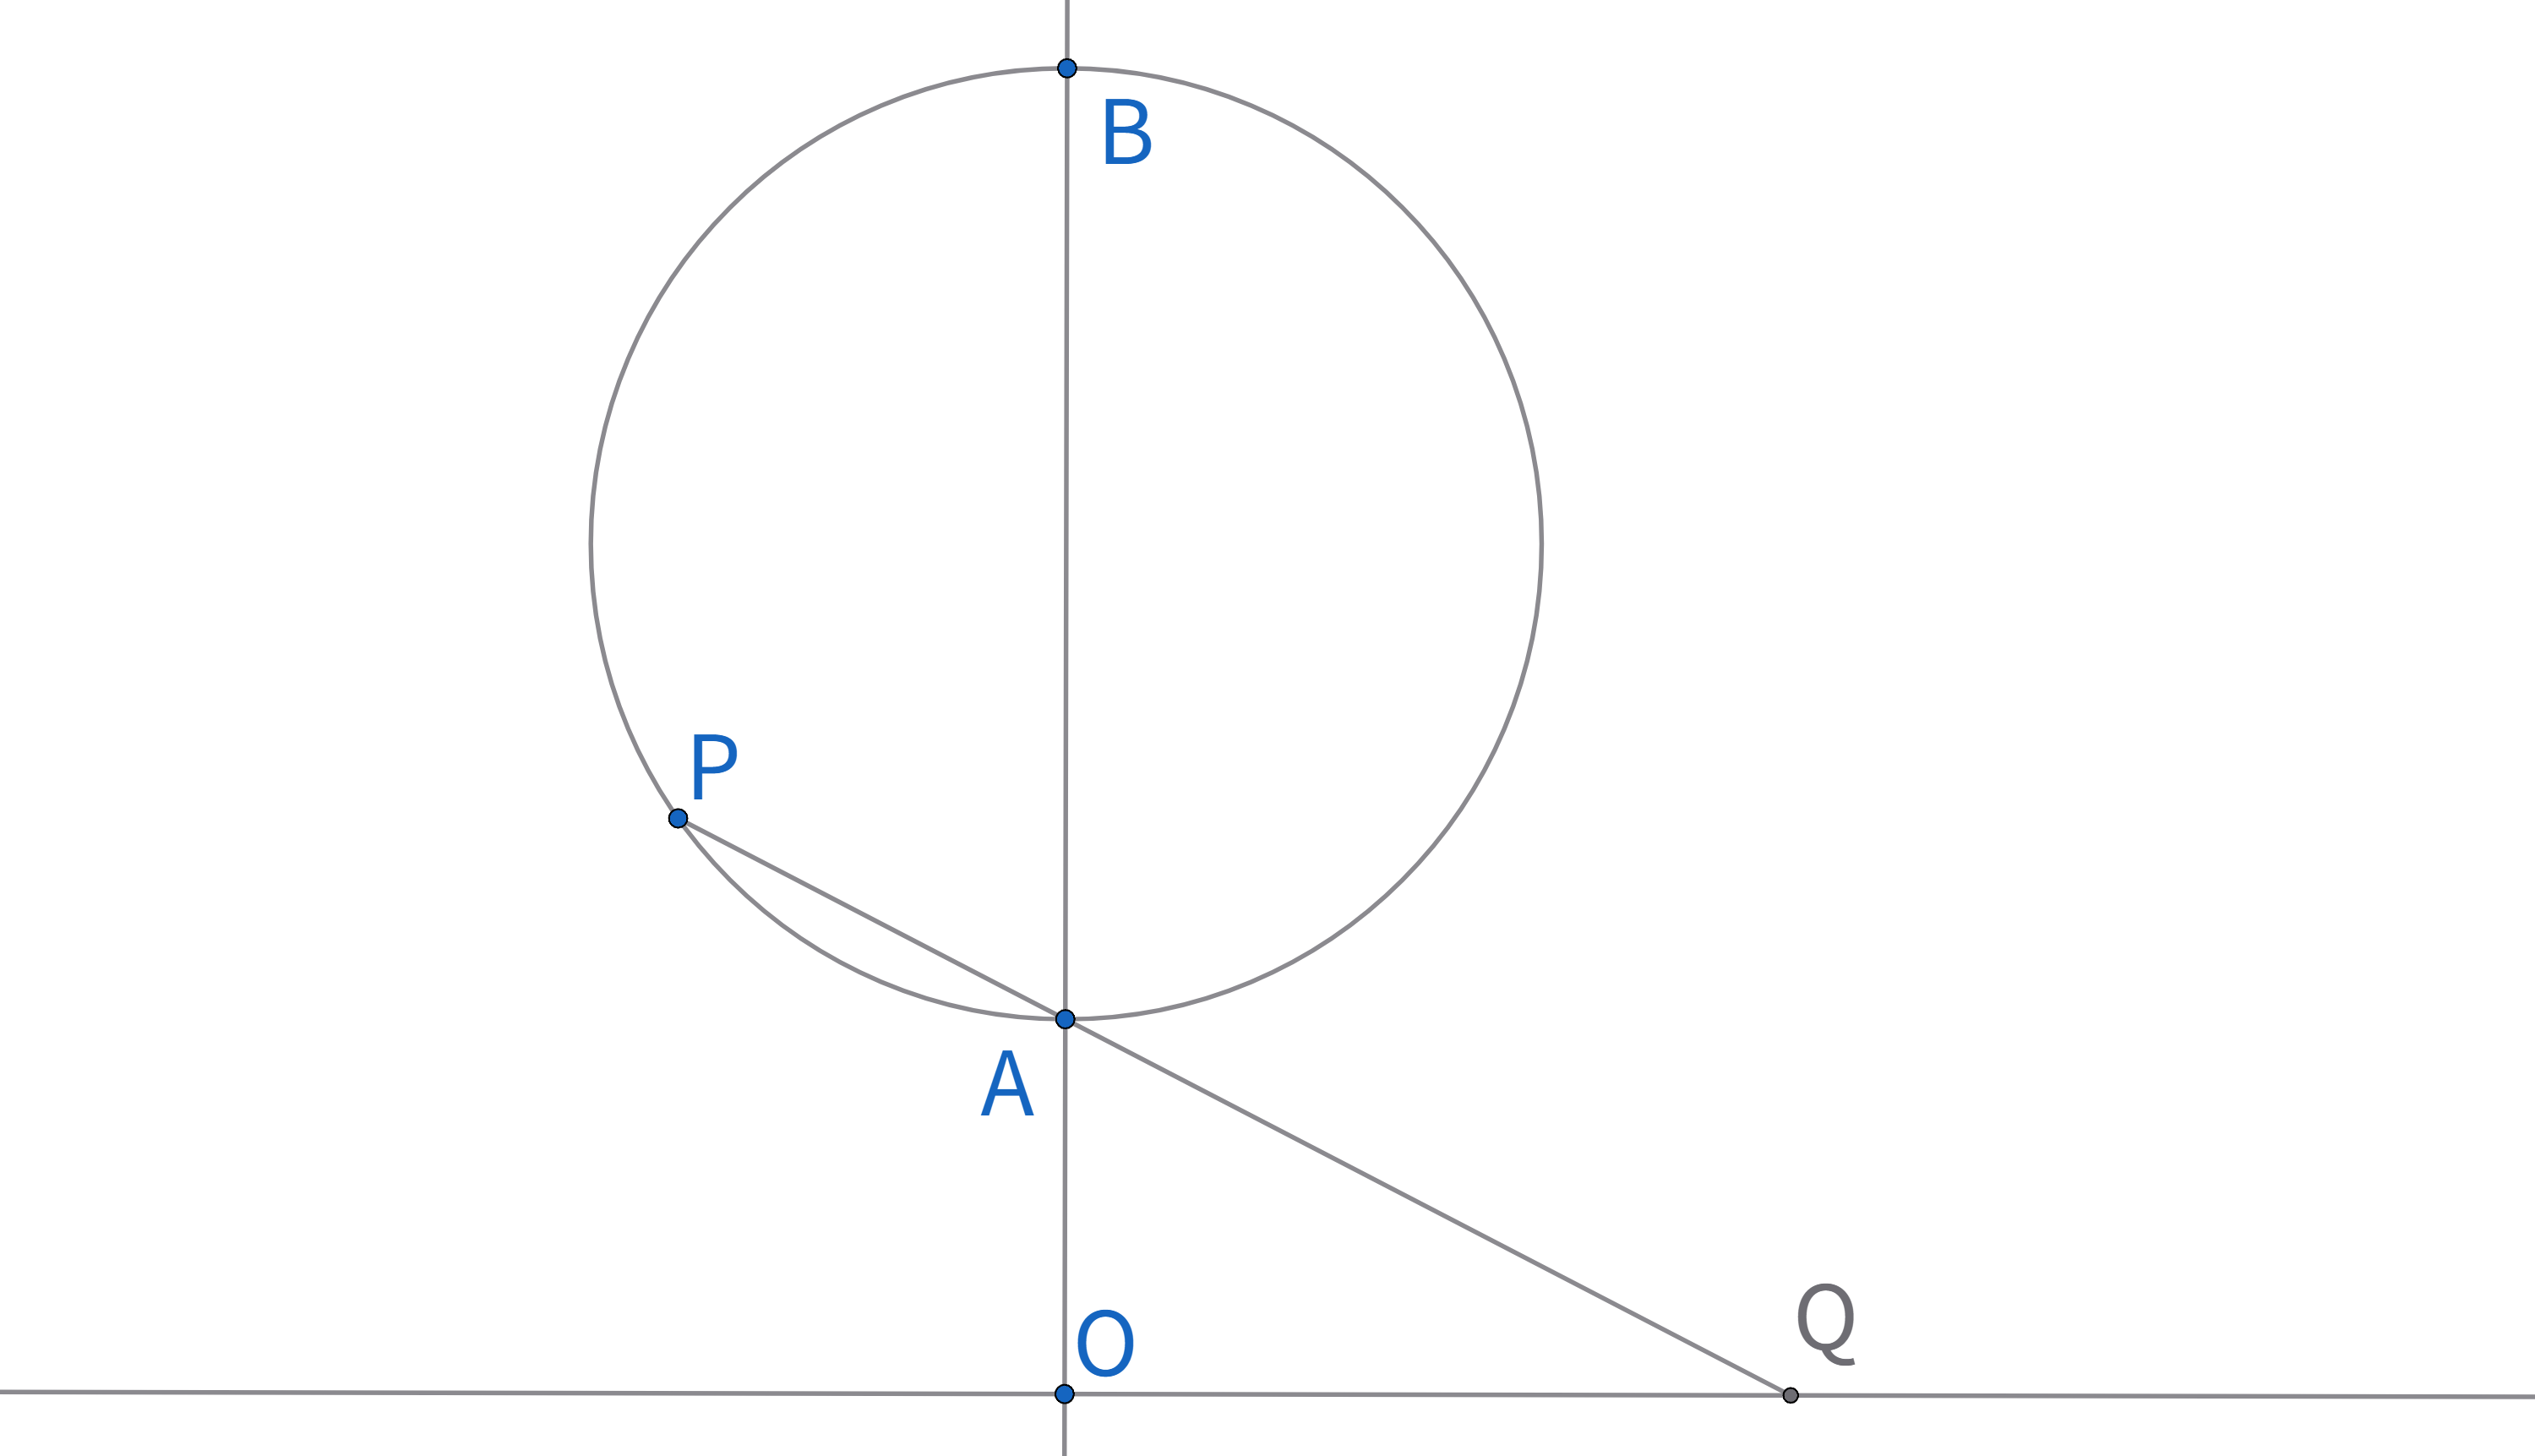
\includegraphics[width=0.7\linewidth]{figures/exercises/003.png}
\end{figure}


\begin{exercise}
在圆内接四边形 $ABCD$ 中,设 $I_1, I_2$ 分别是 $\triangle ABC, \triangle DBC$ 的内心。证明:$I_1, I_2, B, C$ 四点共圆。
\end{exercise}
\begin{figure}[H]
    \centering
    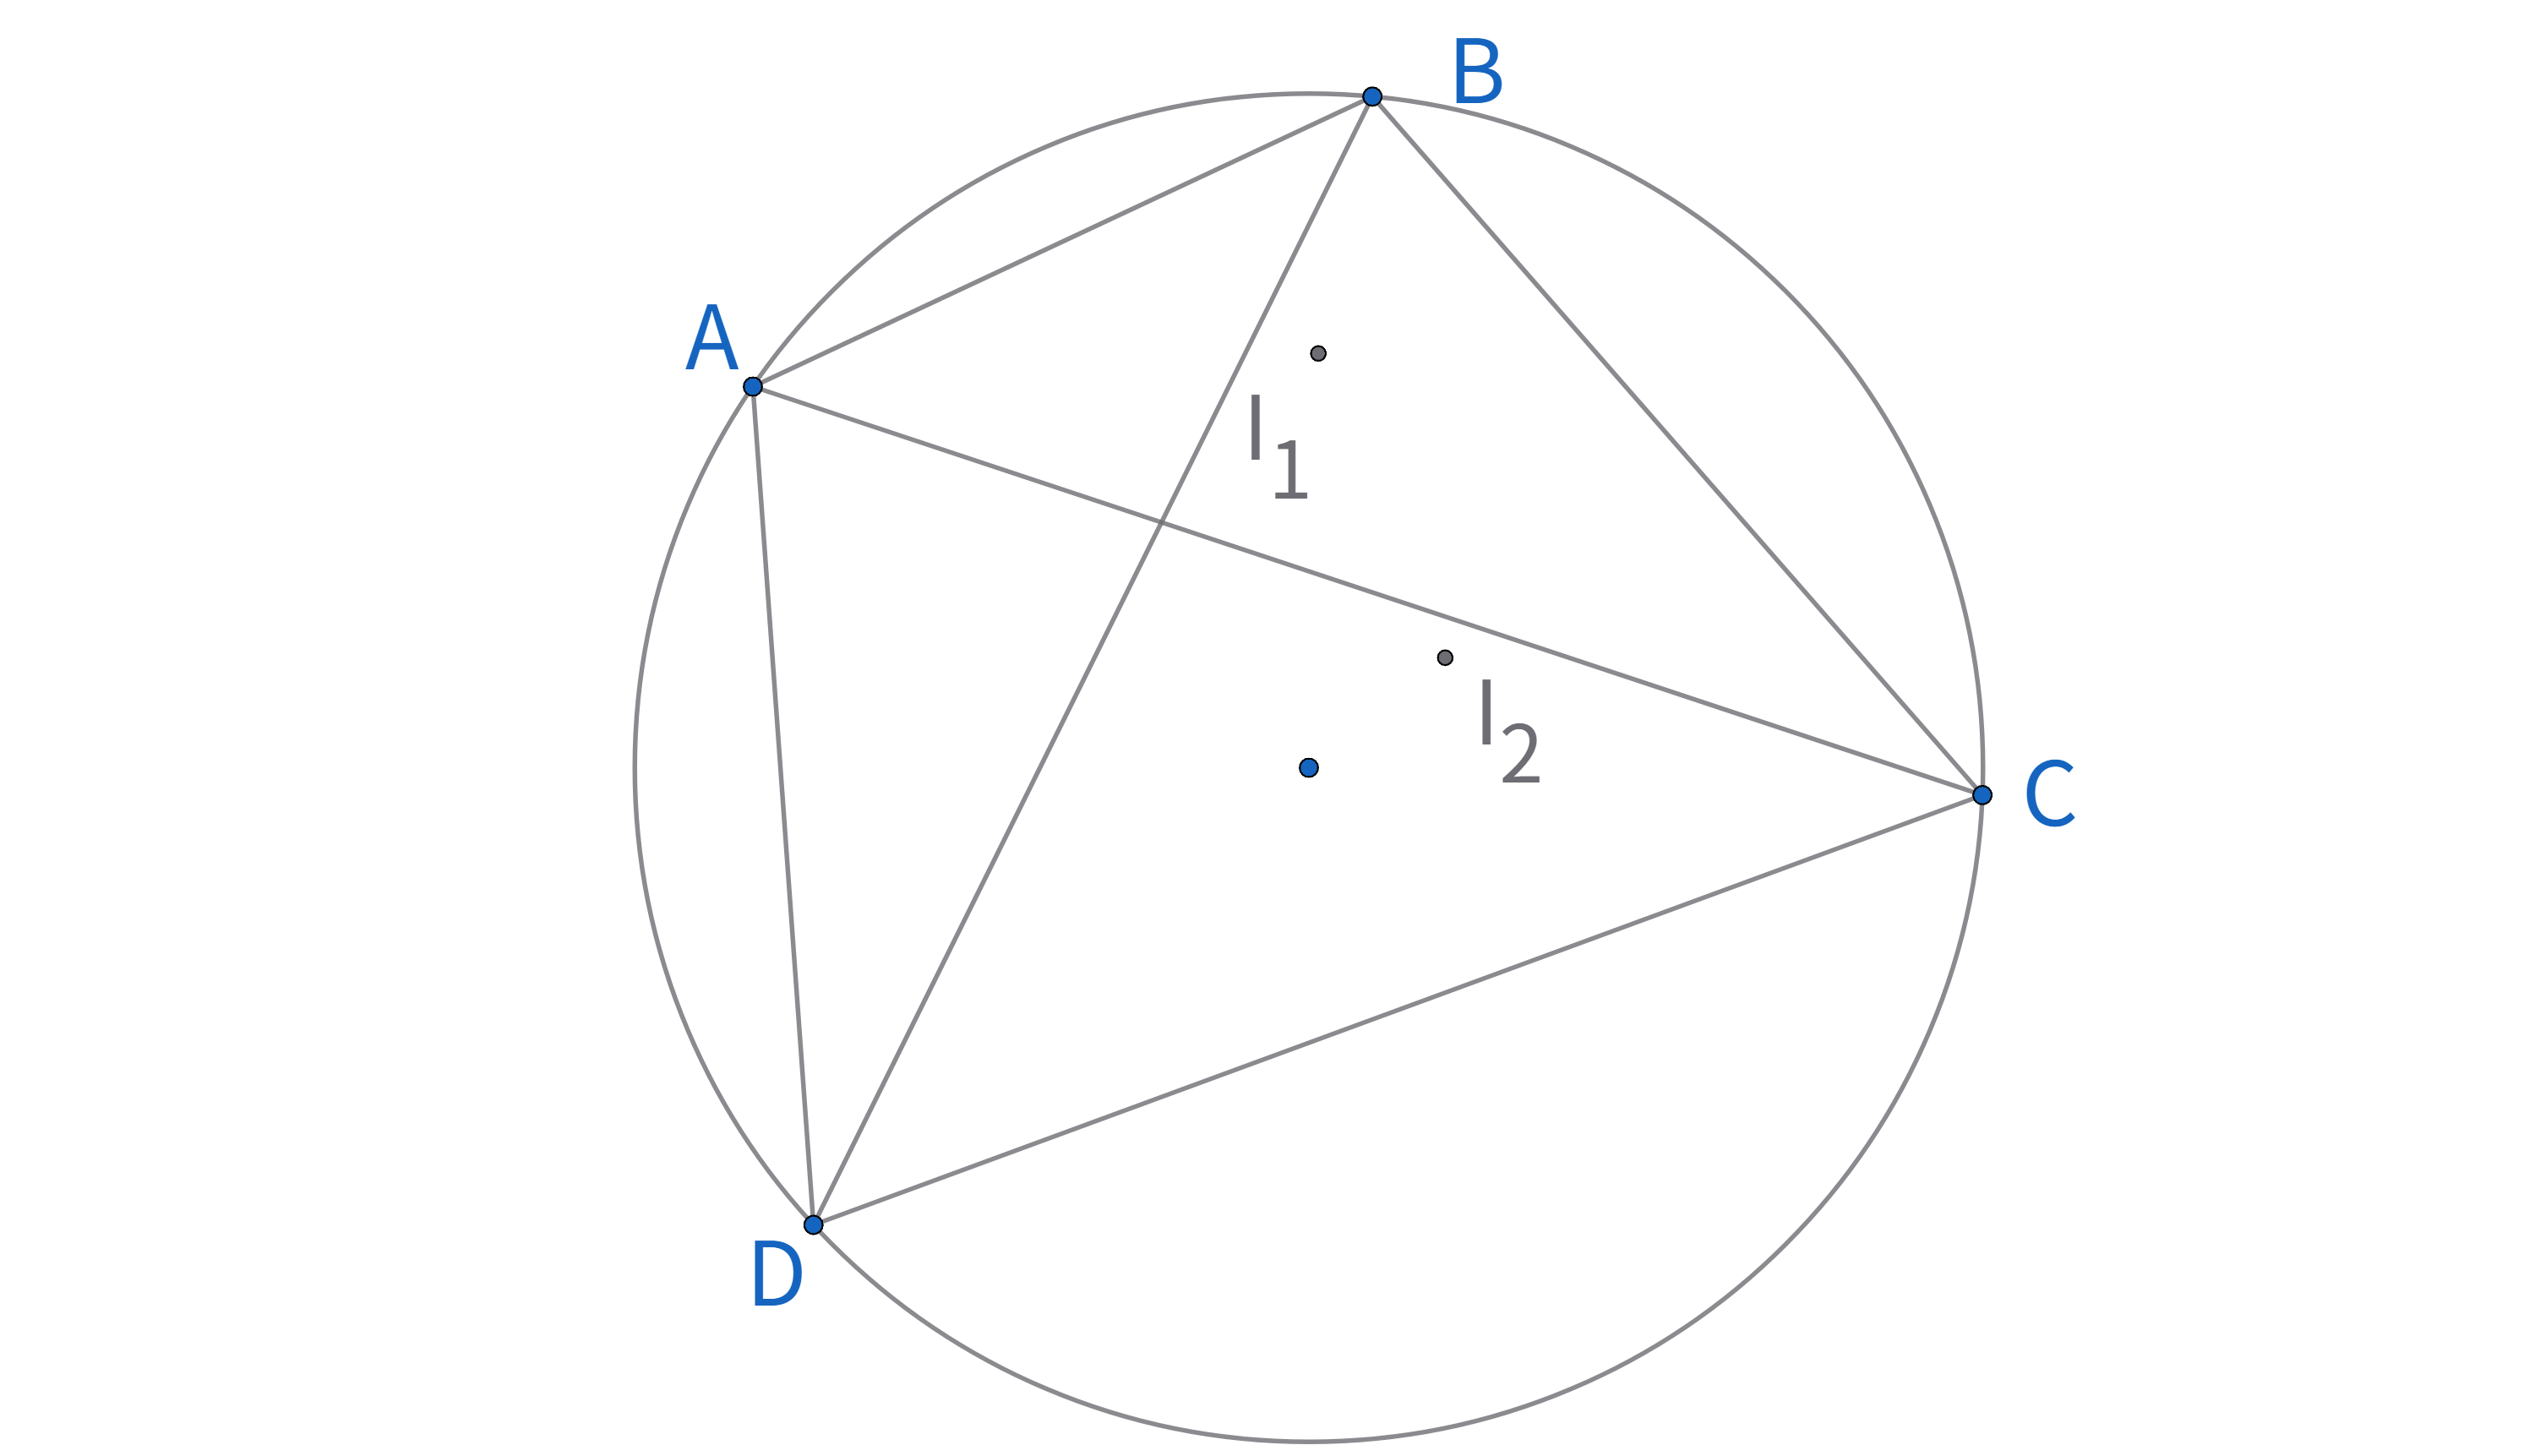
\includegraphics[width=0.7\linewidth]{figures/exercises/004.png}
\end{figure}

\newpage 
\begin{exercise}
(CGMO 2012/5) 设 $\triangle ABC$ 的内切圆分别与边 $AB, AC$ 相切于点 $D, E, O$ 是 $\triangle BCI$ 的外心。证明:$\angle ODB = \angle OEC$。
\end{exercise}
\begin{figure}[H]
    \centering
    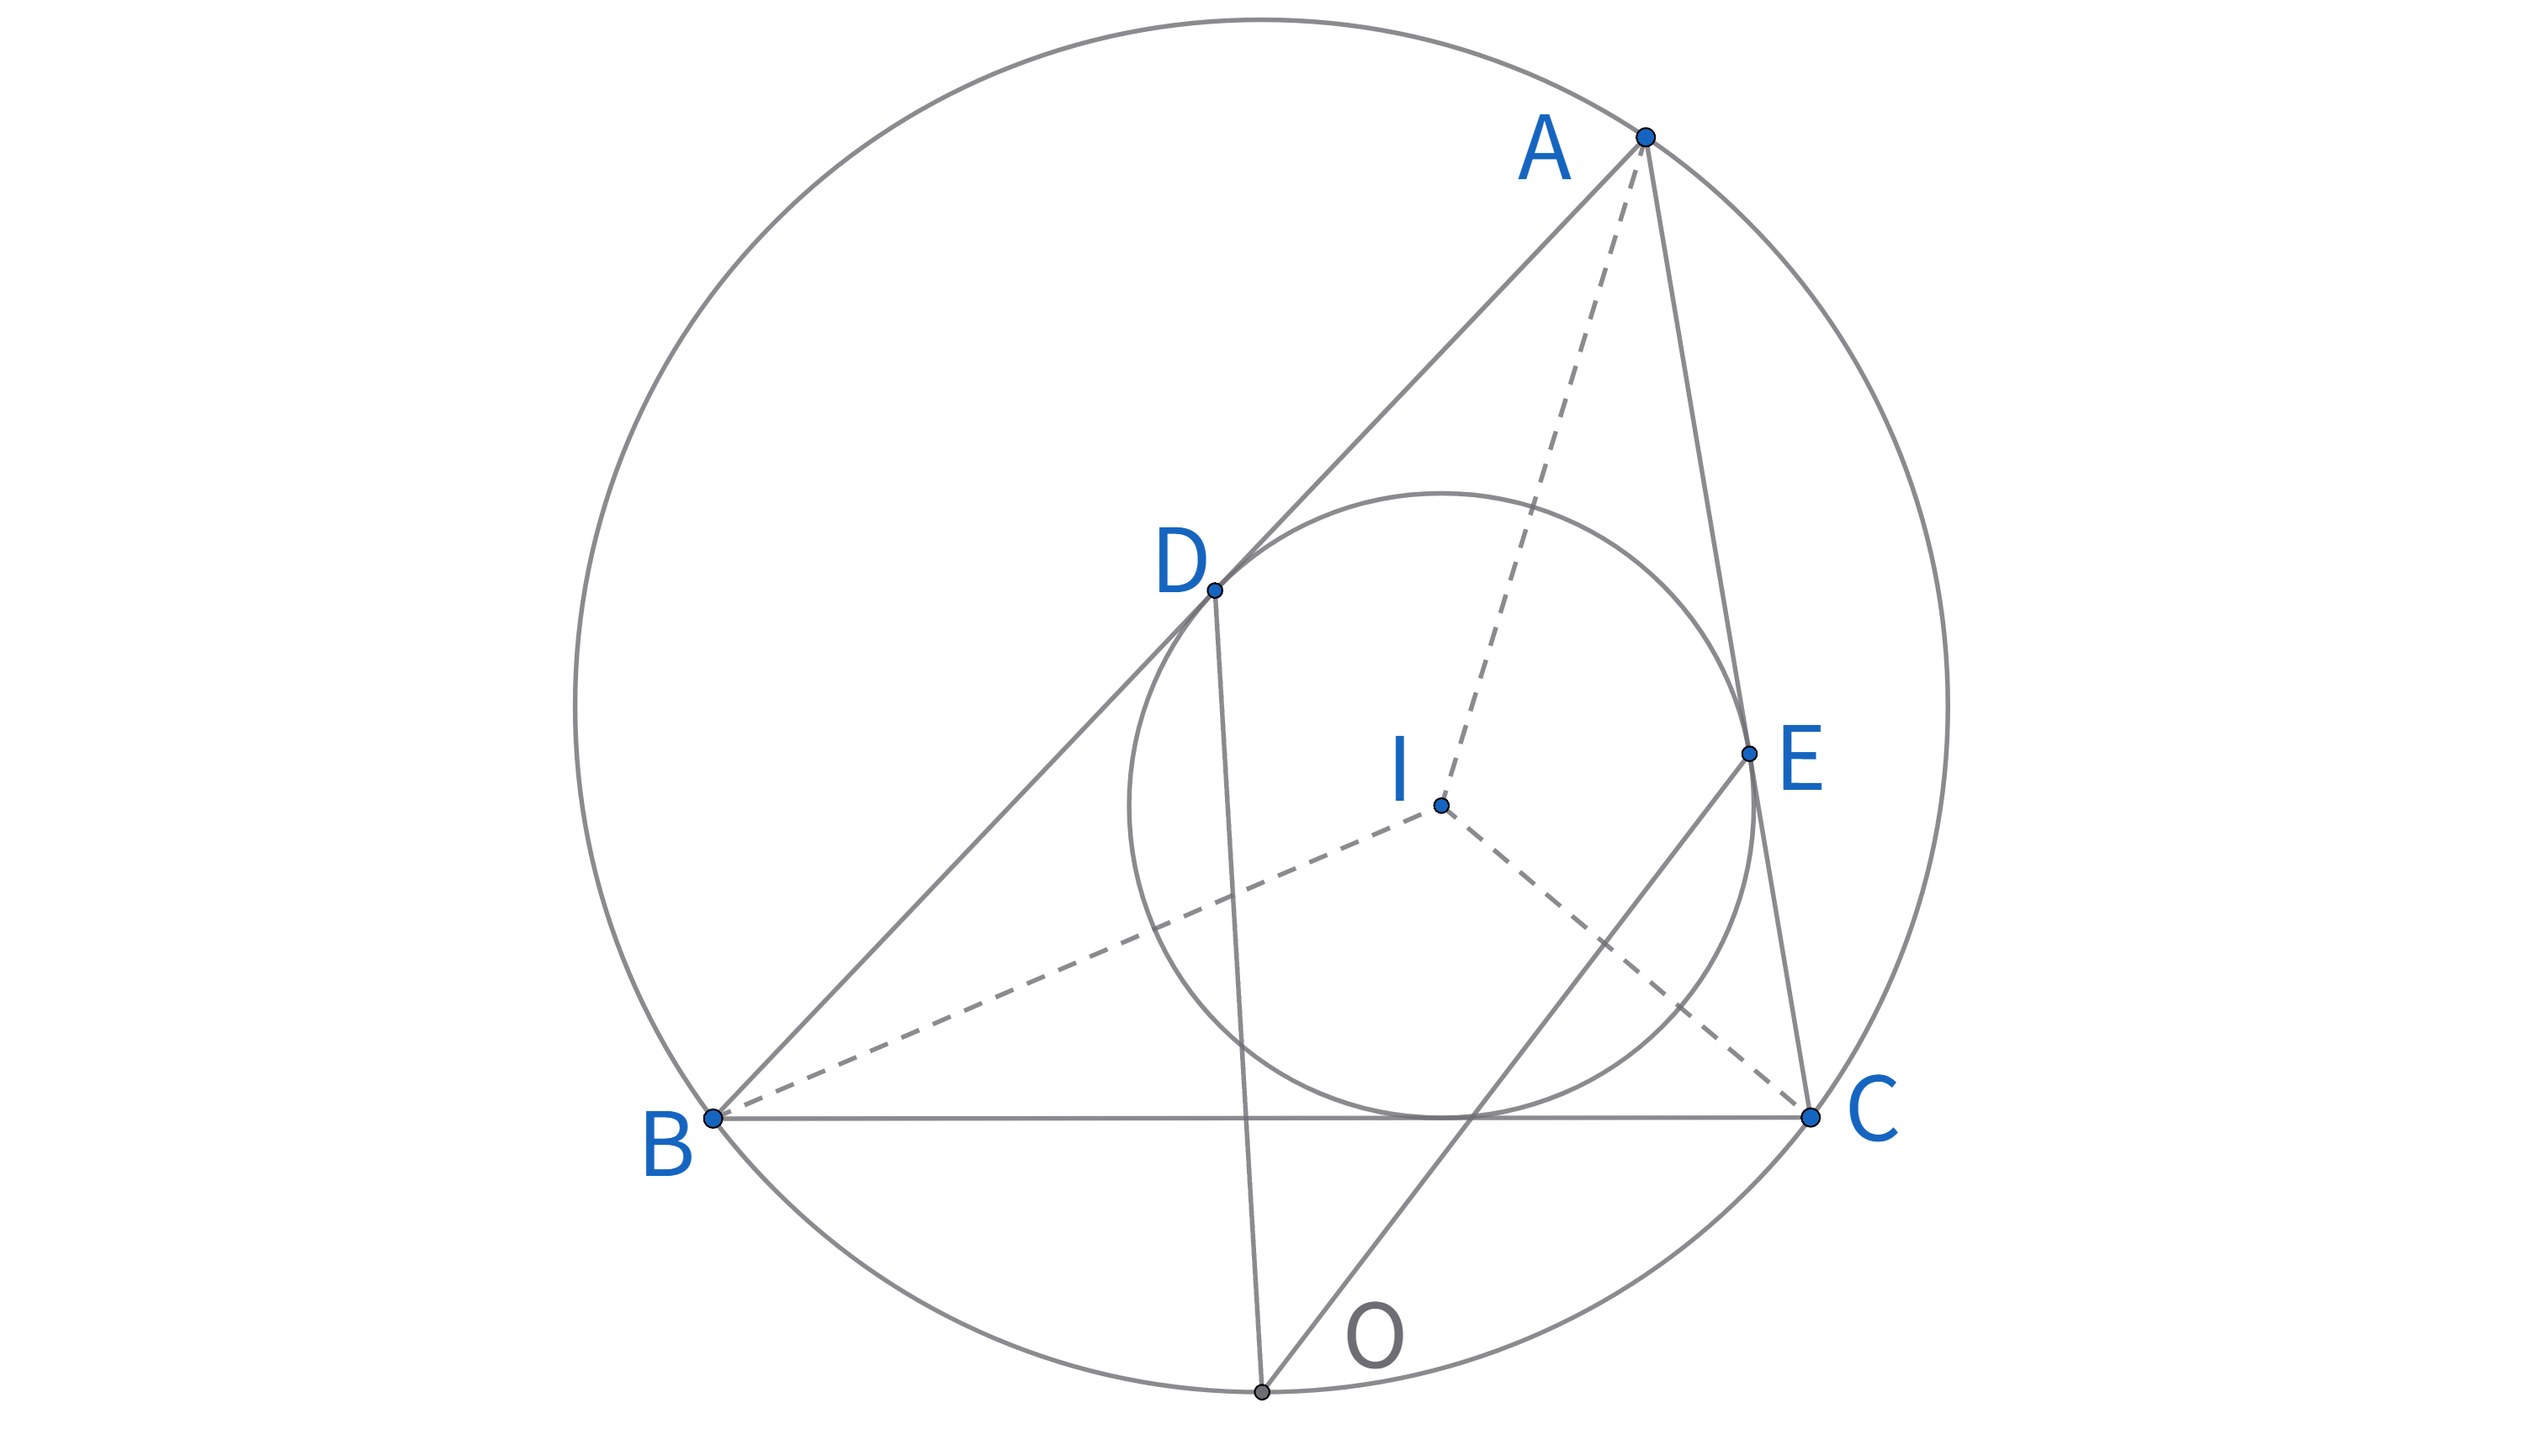
\includegraphics[width=0.7\linewidth]{figures/exercises/005.png}
\end{figure}


\begin{exercise}
(加拿大 1991/3) 设 $P$ 是圆 $\omega$ 内一点,考虑 $\omega$ 的所有经过 $P$ 的弦。证明:这些弦的中点都在一个圆上。
\end{exercise}


\begin{exercise}
(俄罗斯 1996) 点 $E$ 和 $F$ 在凸四边形 $ABCD$ 的边 $BC$ 上($E$ 在 $B$ 和 $F$ 之间)。已知 $\angle BAE = \angle CDF$,且 $\angle EAF = \angle FDE$。证明:$\angle FAC = \angle EDB$。
\end{exercise}
\begin{figure}[H]
    \centering
    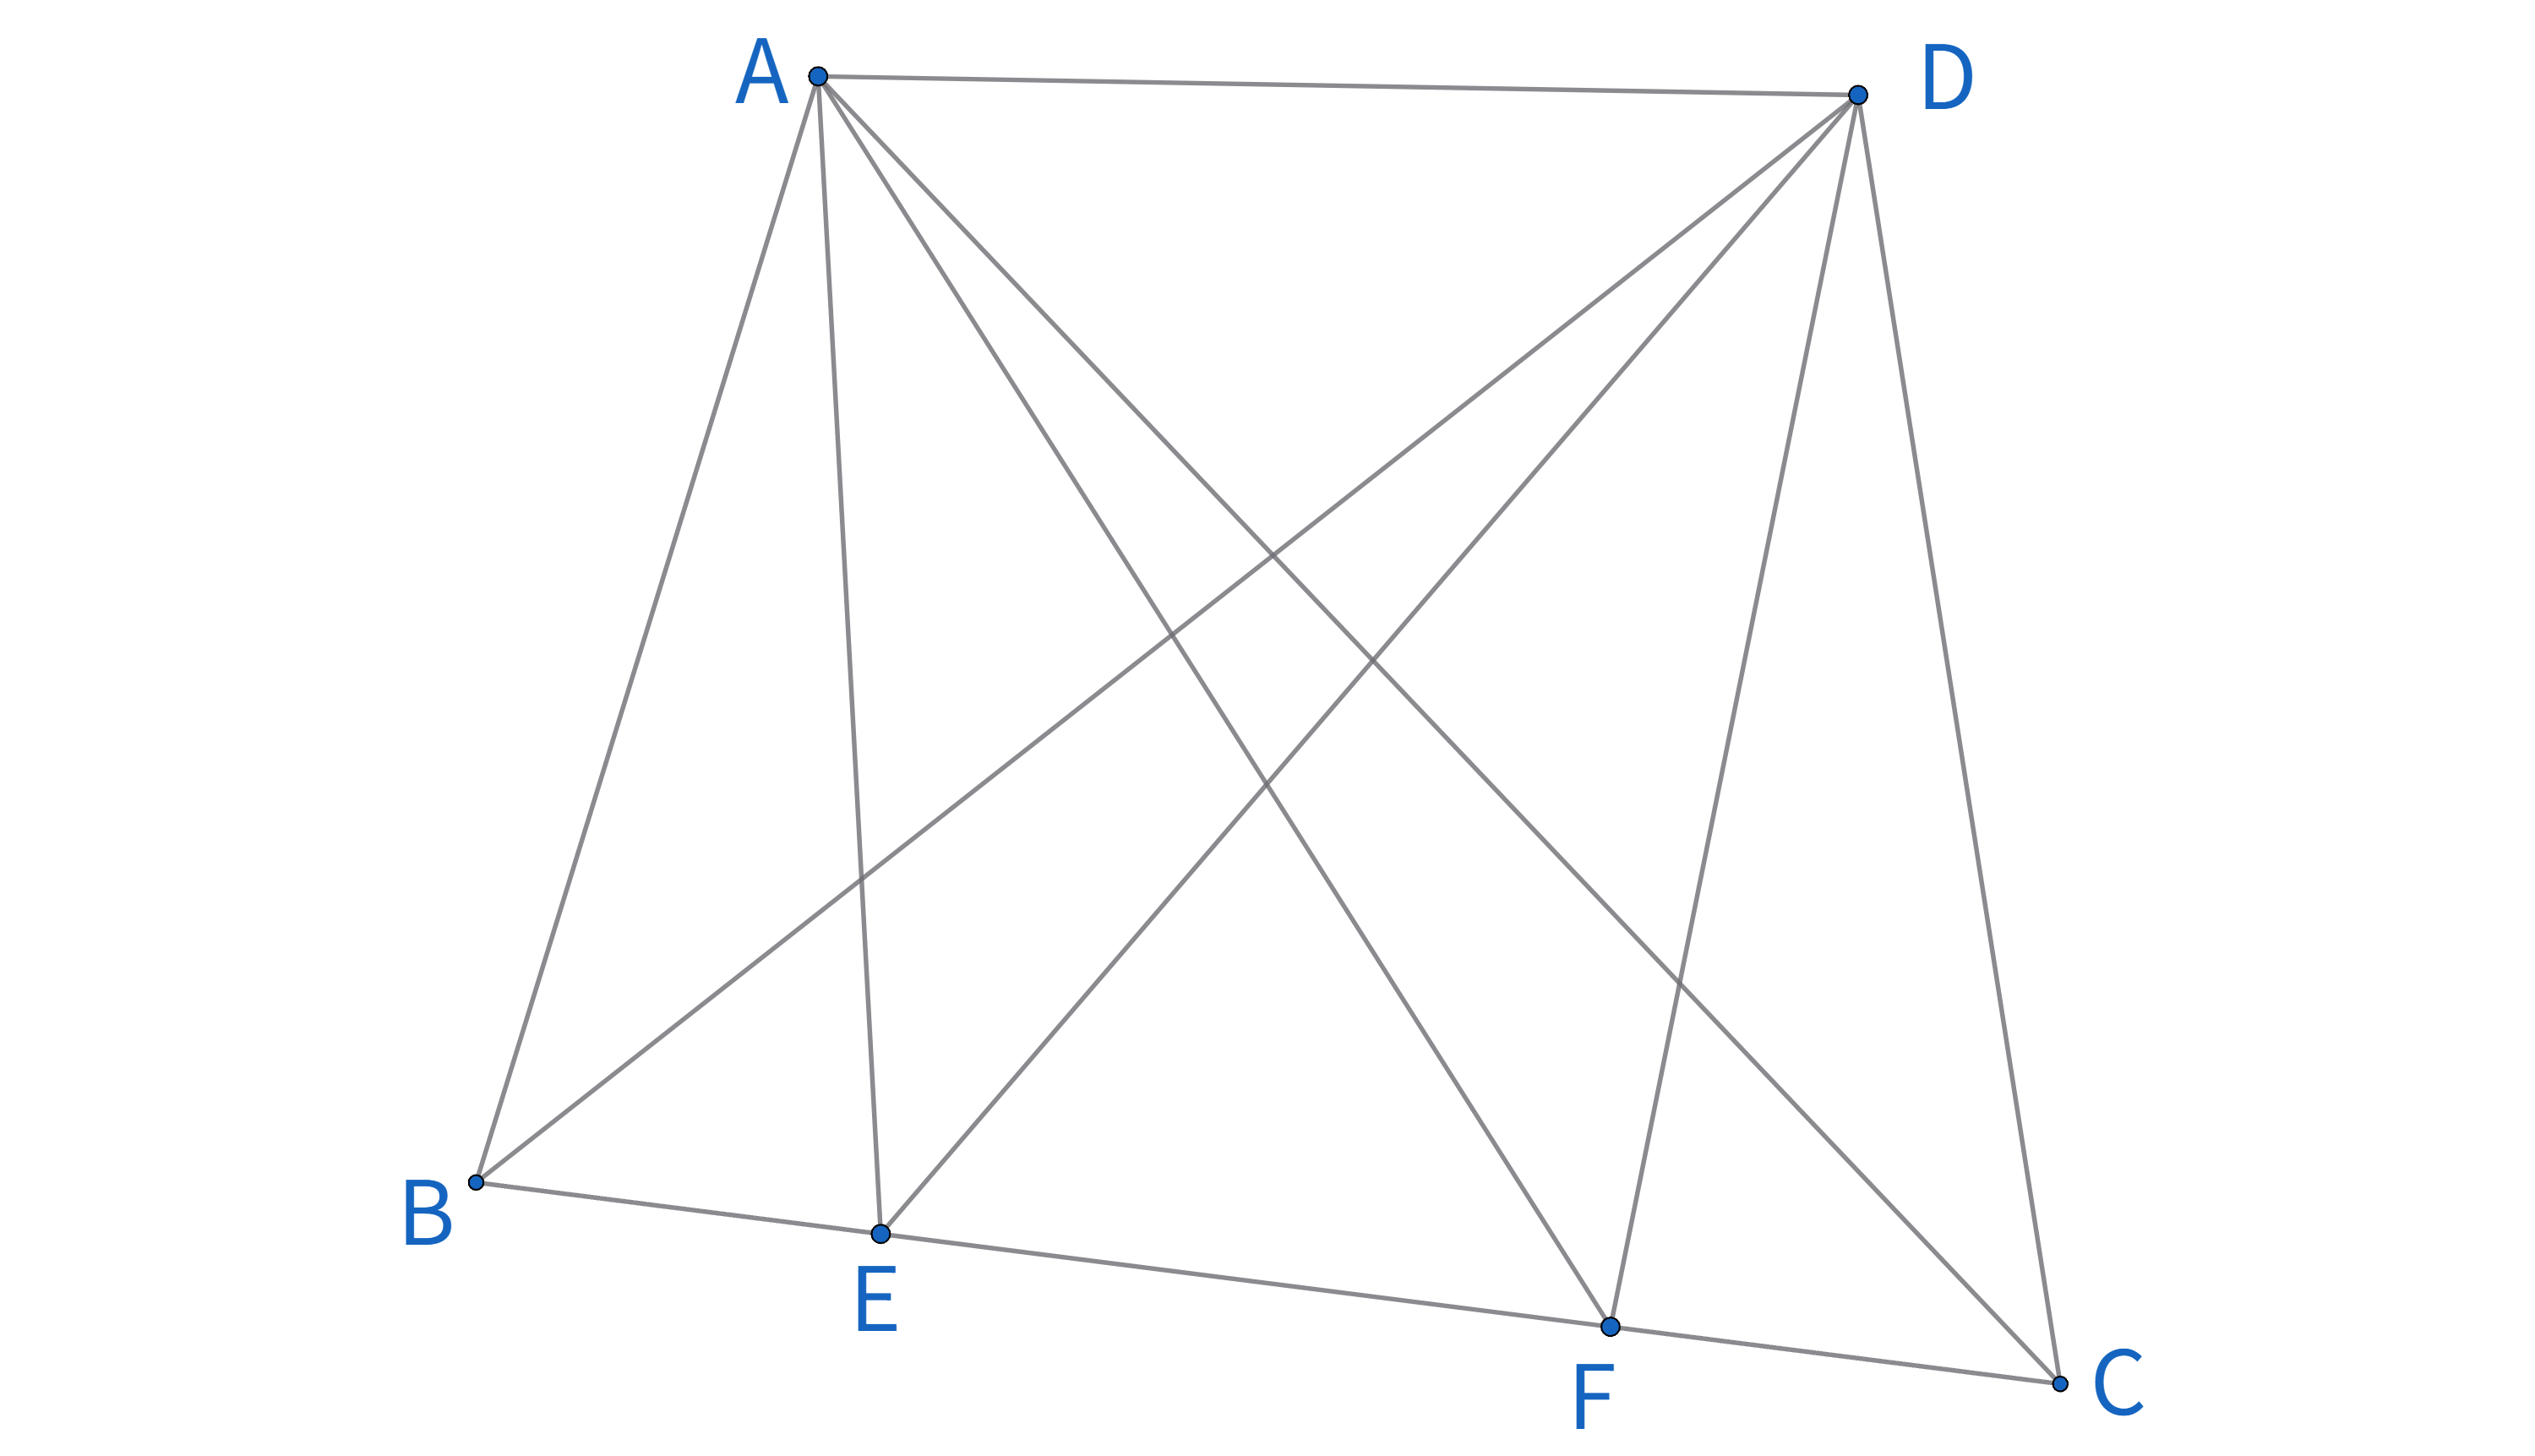
\includegraphics[width=0.7\linewidth]{figures/exercises/006.png}
\end{figure}

\newpage 
\begin{exercise}
设锐角 $\triangle ABC$ 的外接圆为 $\Gamma$,$X$ 是劣弧 $\overset{\frown}{BC}$ 的中点,类似地定义 $Y, Z$,证明:$\triangle XYZ$ 的垂心是 $\triangle ABC$ 的内心。
\end{exercise}
\begin{figure}[H]
    \centering
    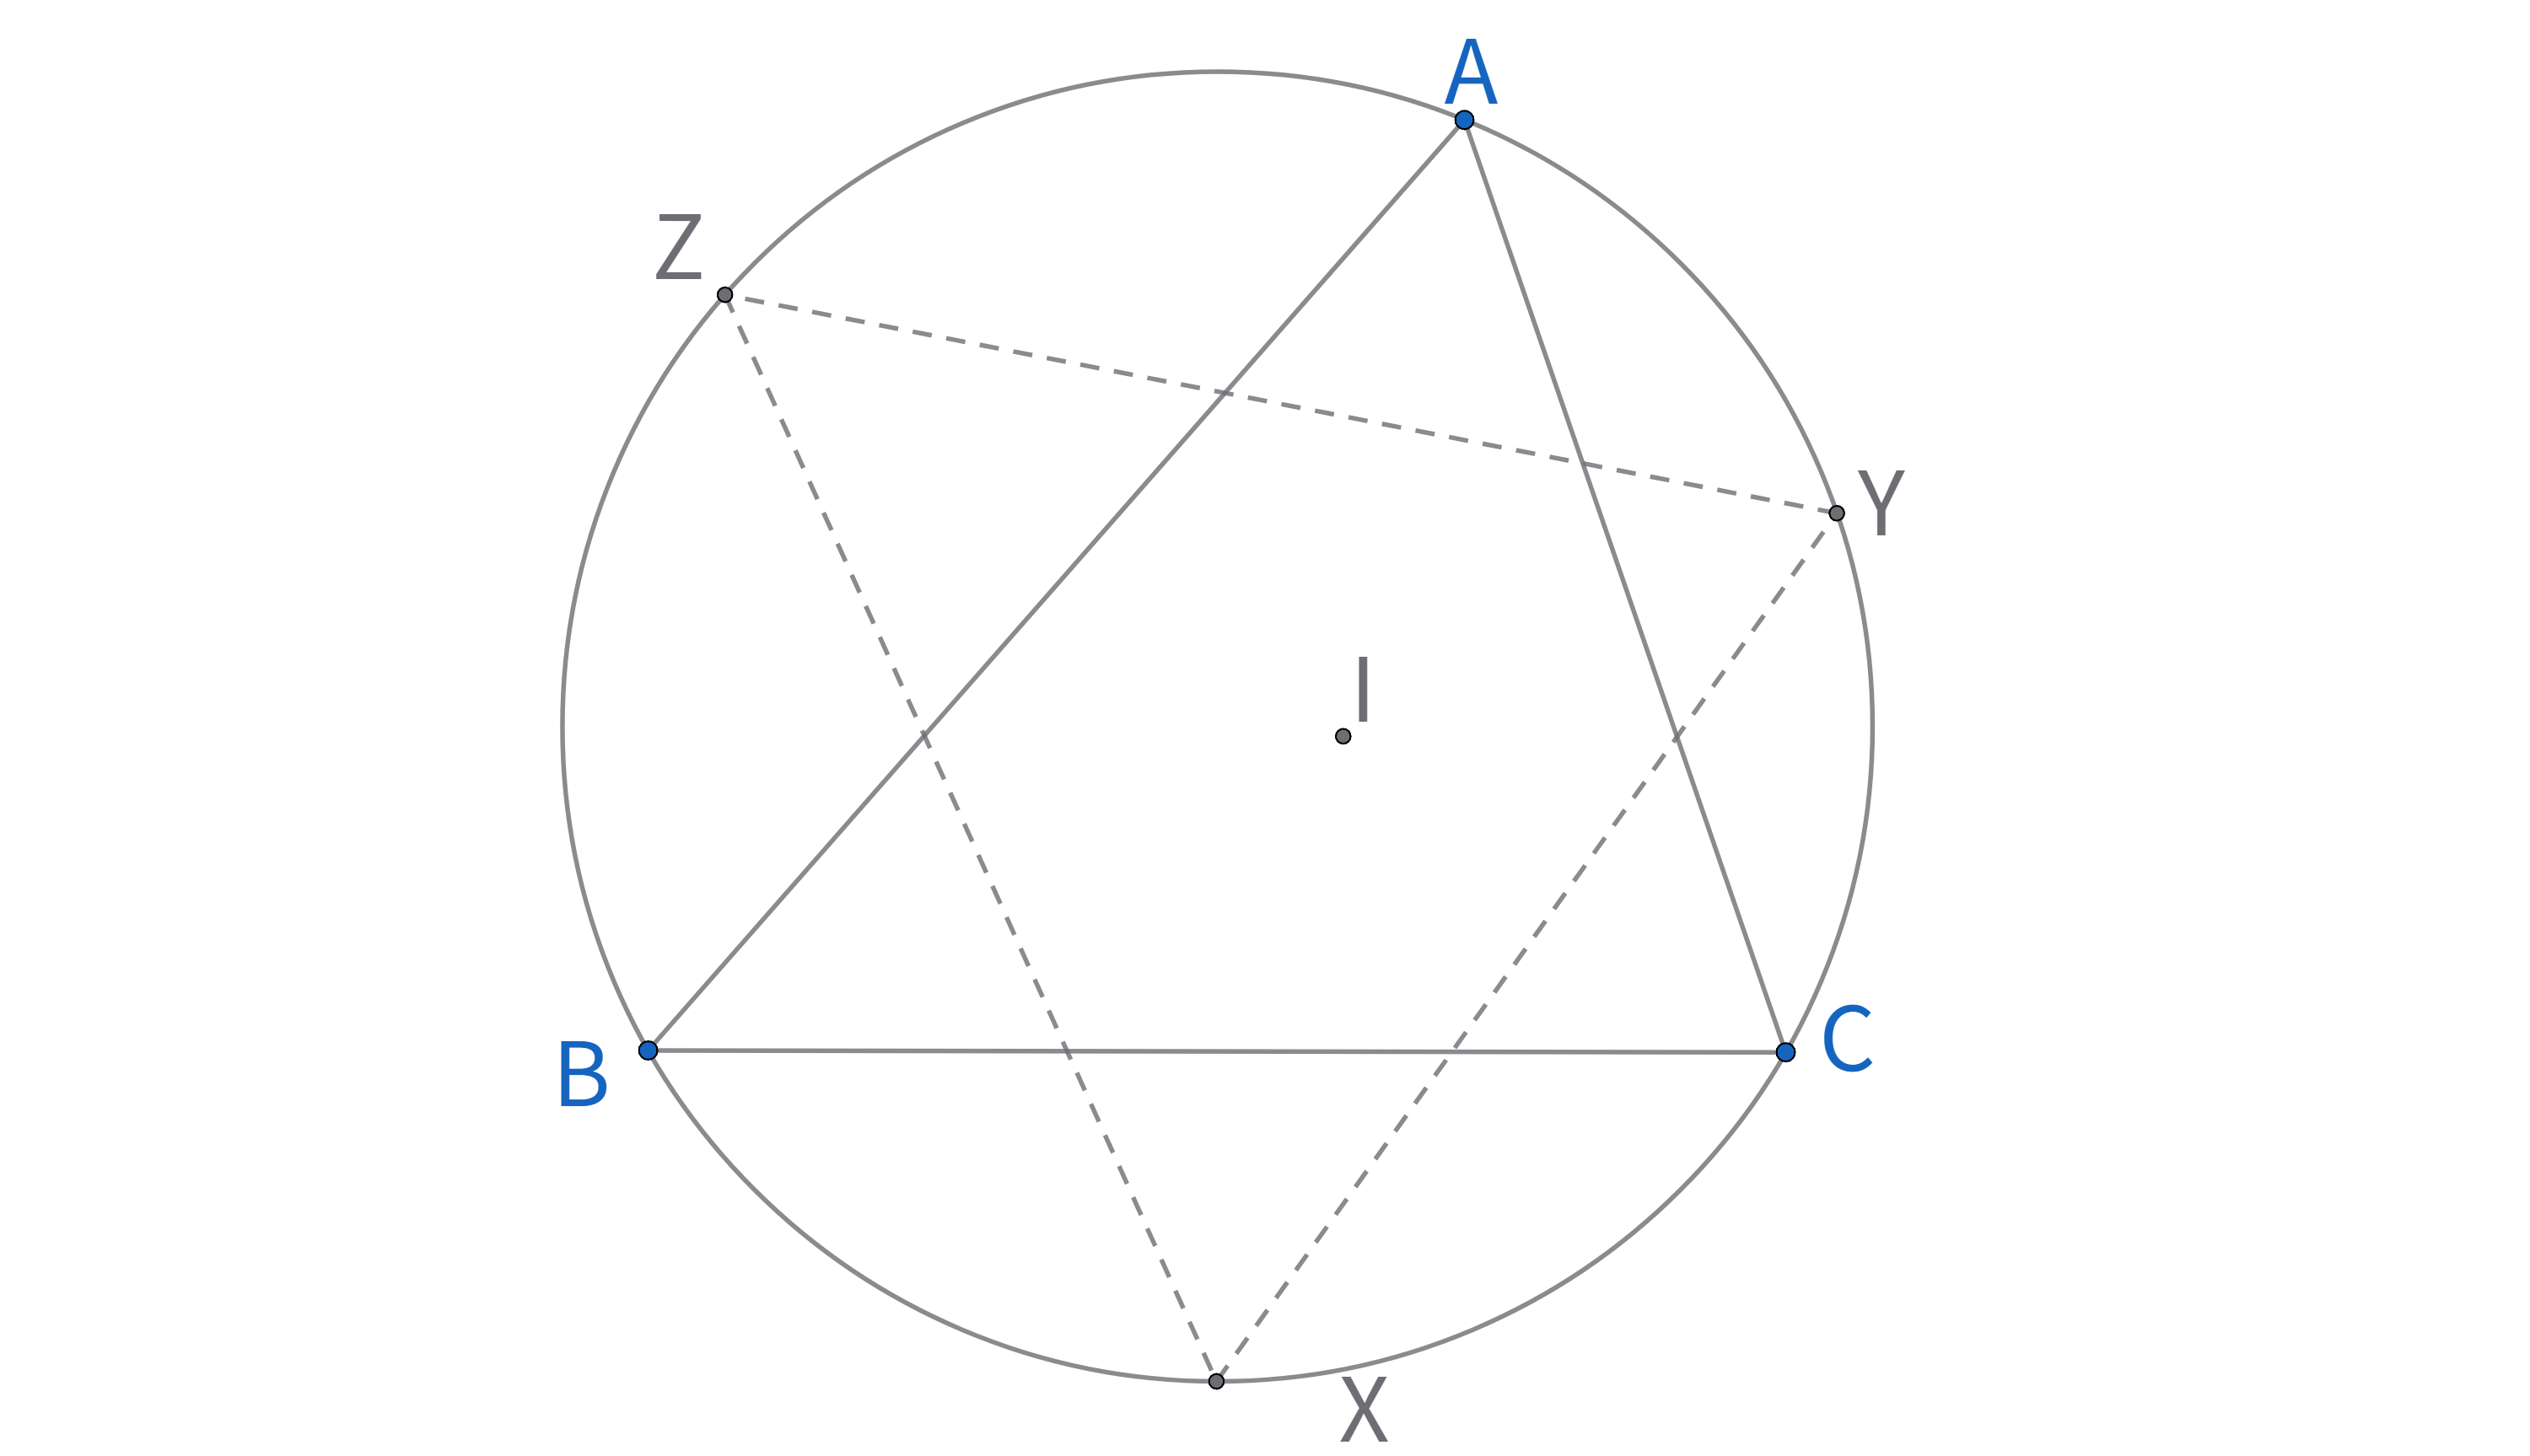
\includegraphics[width=0.7\linewidth]{figures/exercises/007.png}
\end{figure}


\begin{exercise}
(JMO 2011/5) 点 $A, B, C, D, E$ 在圆 $\omega$ 上,而点 $P$ 在圆 $\omega$ 外。这些点满足:(i) 直线 $PB, PD$ 与圆 $\omega$ 相切;(ii) $P, A, C$ 共线;(iii) $DE \parallel AC$。证明:$BE$ 平分 ${AC}$。
\end{exercise}
\begin{figure}[H]
    \centering
    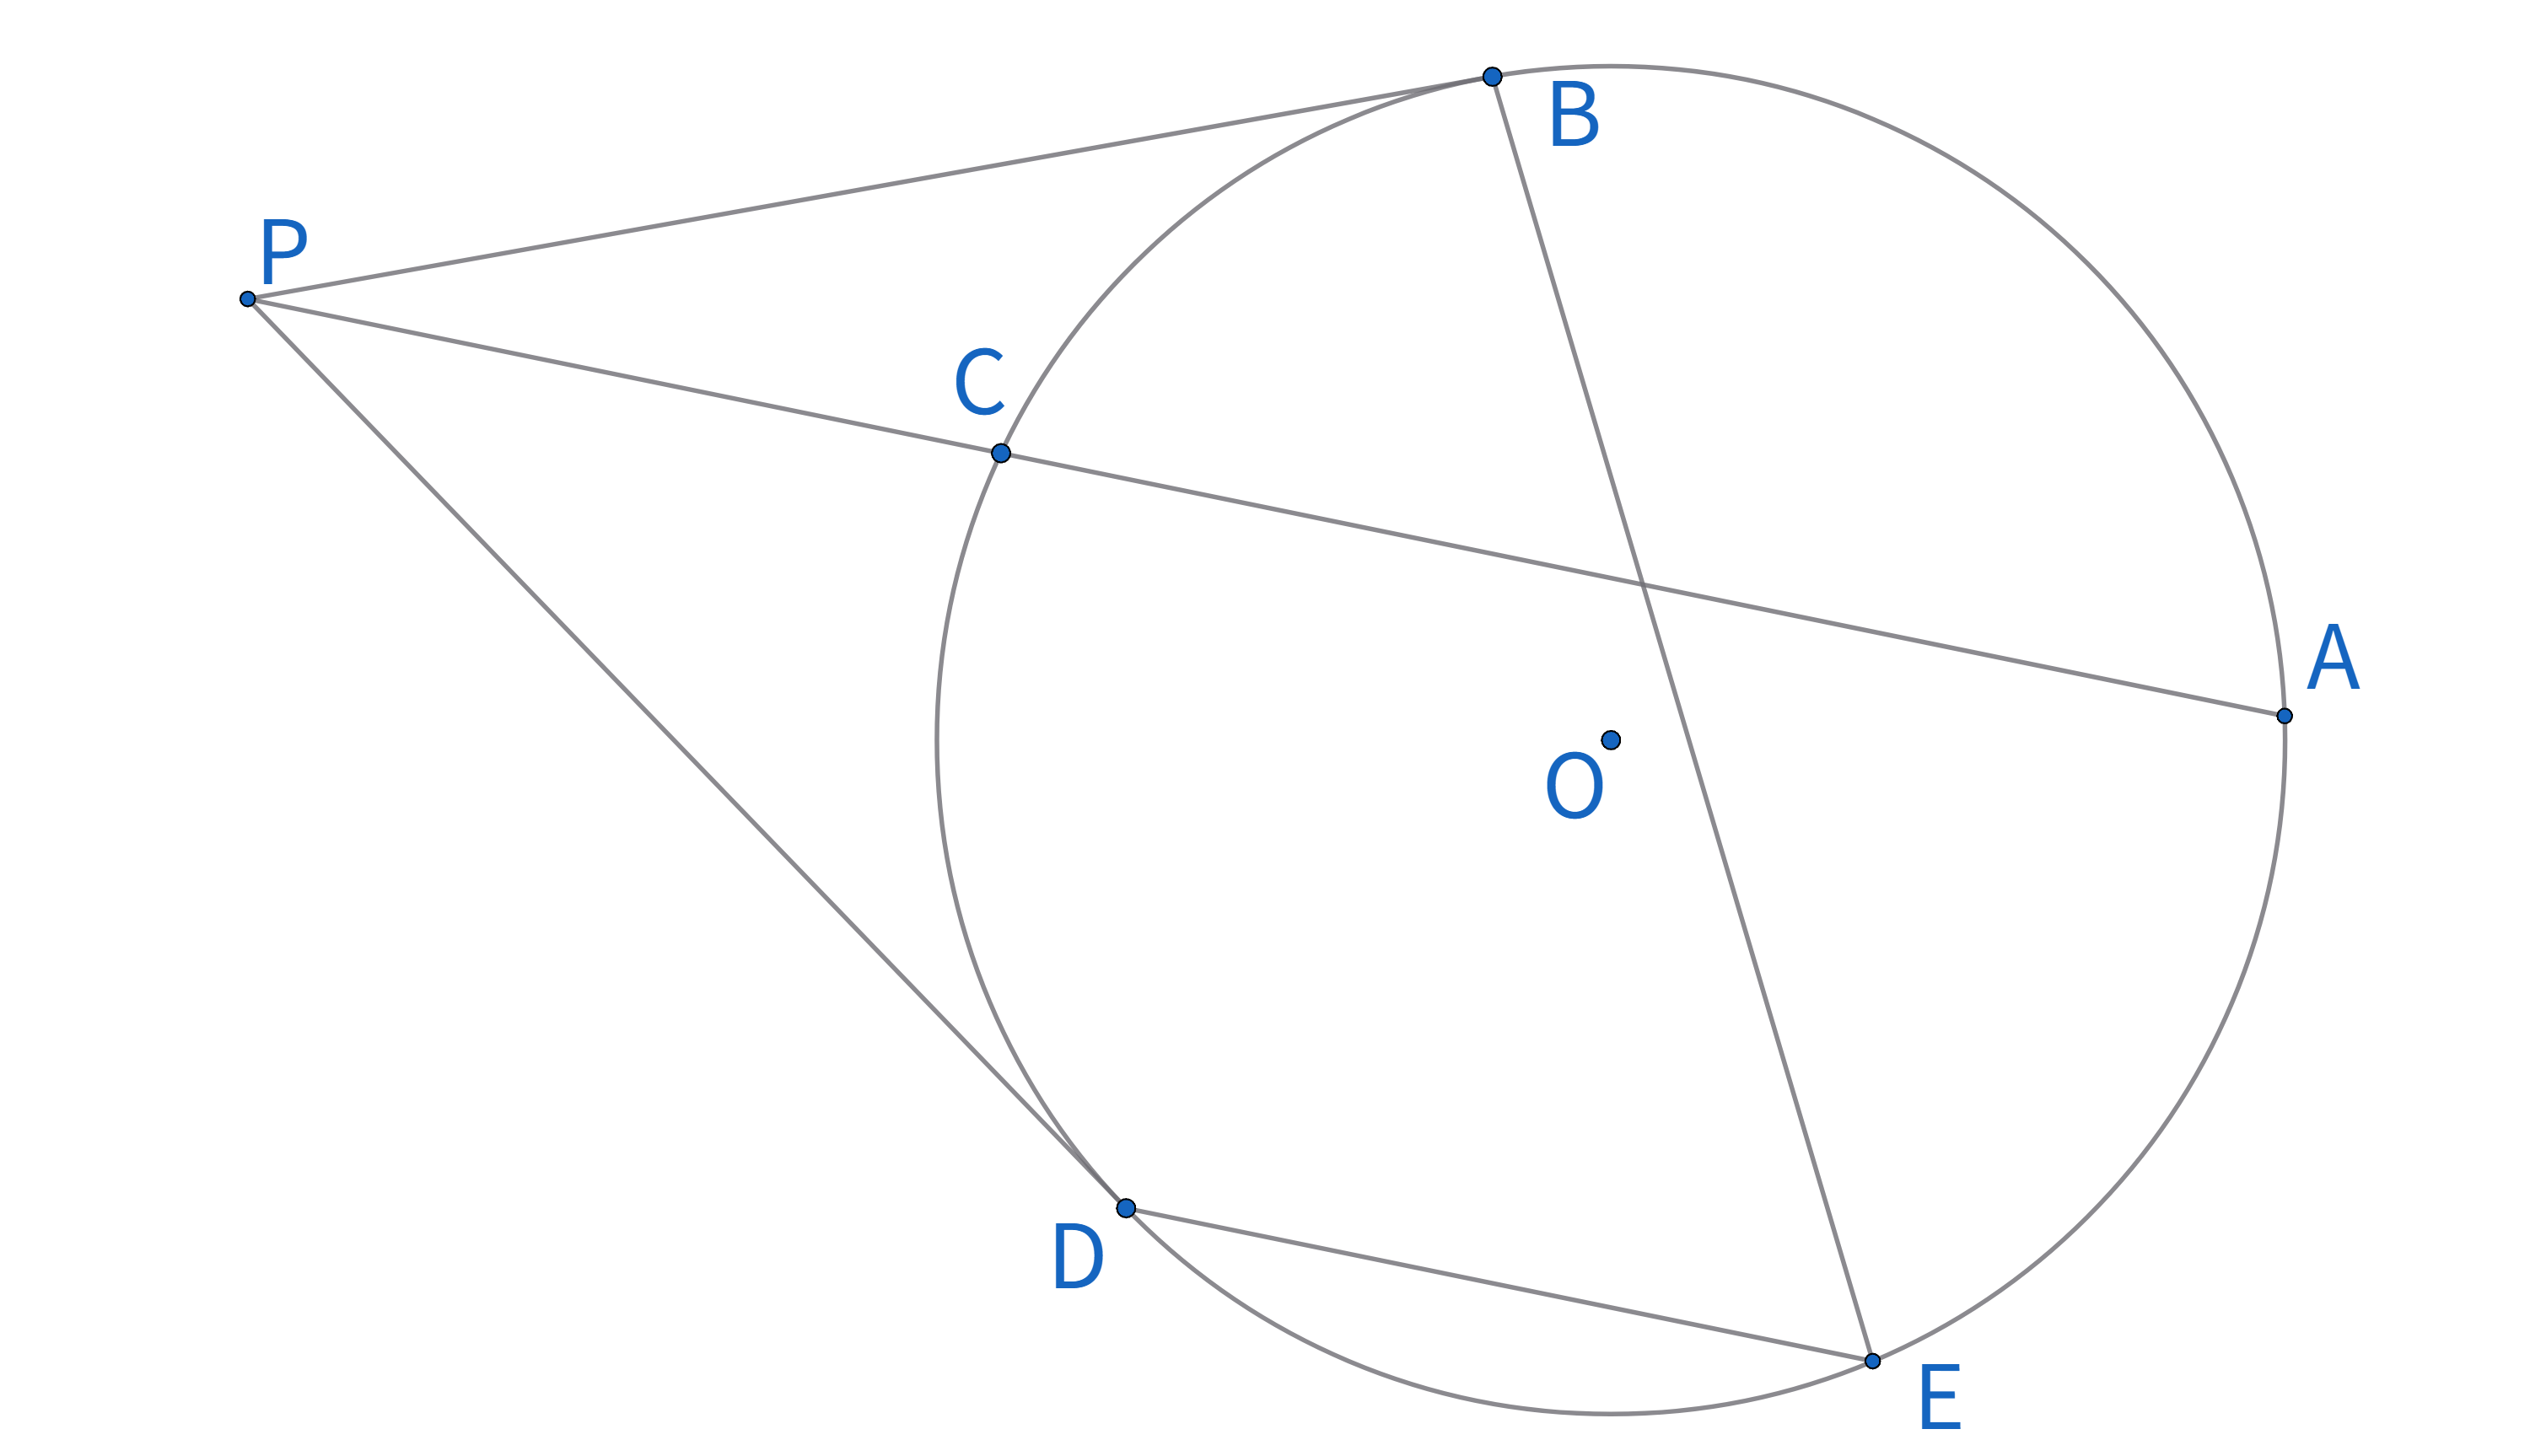
\includegraphics[width=0.7\linewidth]{figures/exercises/008.png}
\end{figure}

\newpage 
\begin{exercise}
设锐角 $\triangle ABC$ 中,$BE, CF$ 是高,$D$ 是 ${BC}$ 的中点。证明:$DE, DF$ 和过 $A$ 与 ${BC}$ 平行的直线均与圆 $(AEF)$ 相切。
\end{exercise}
\begin{figure}[H]
    \centering
    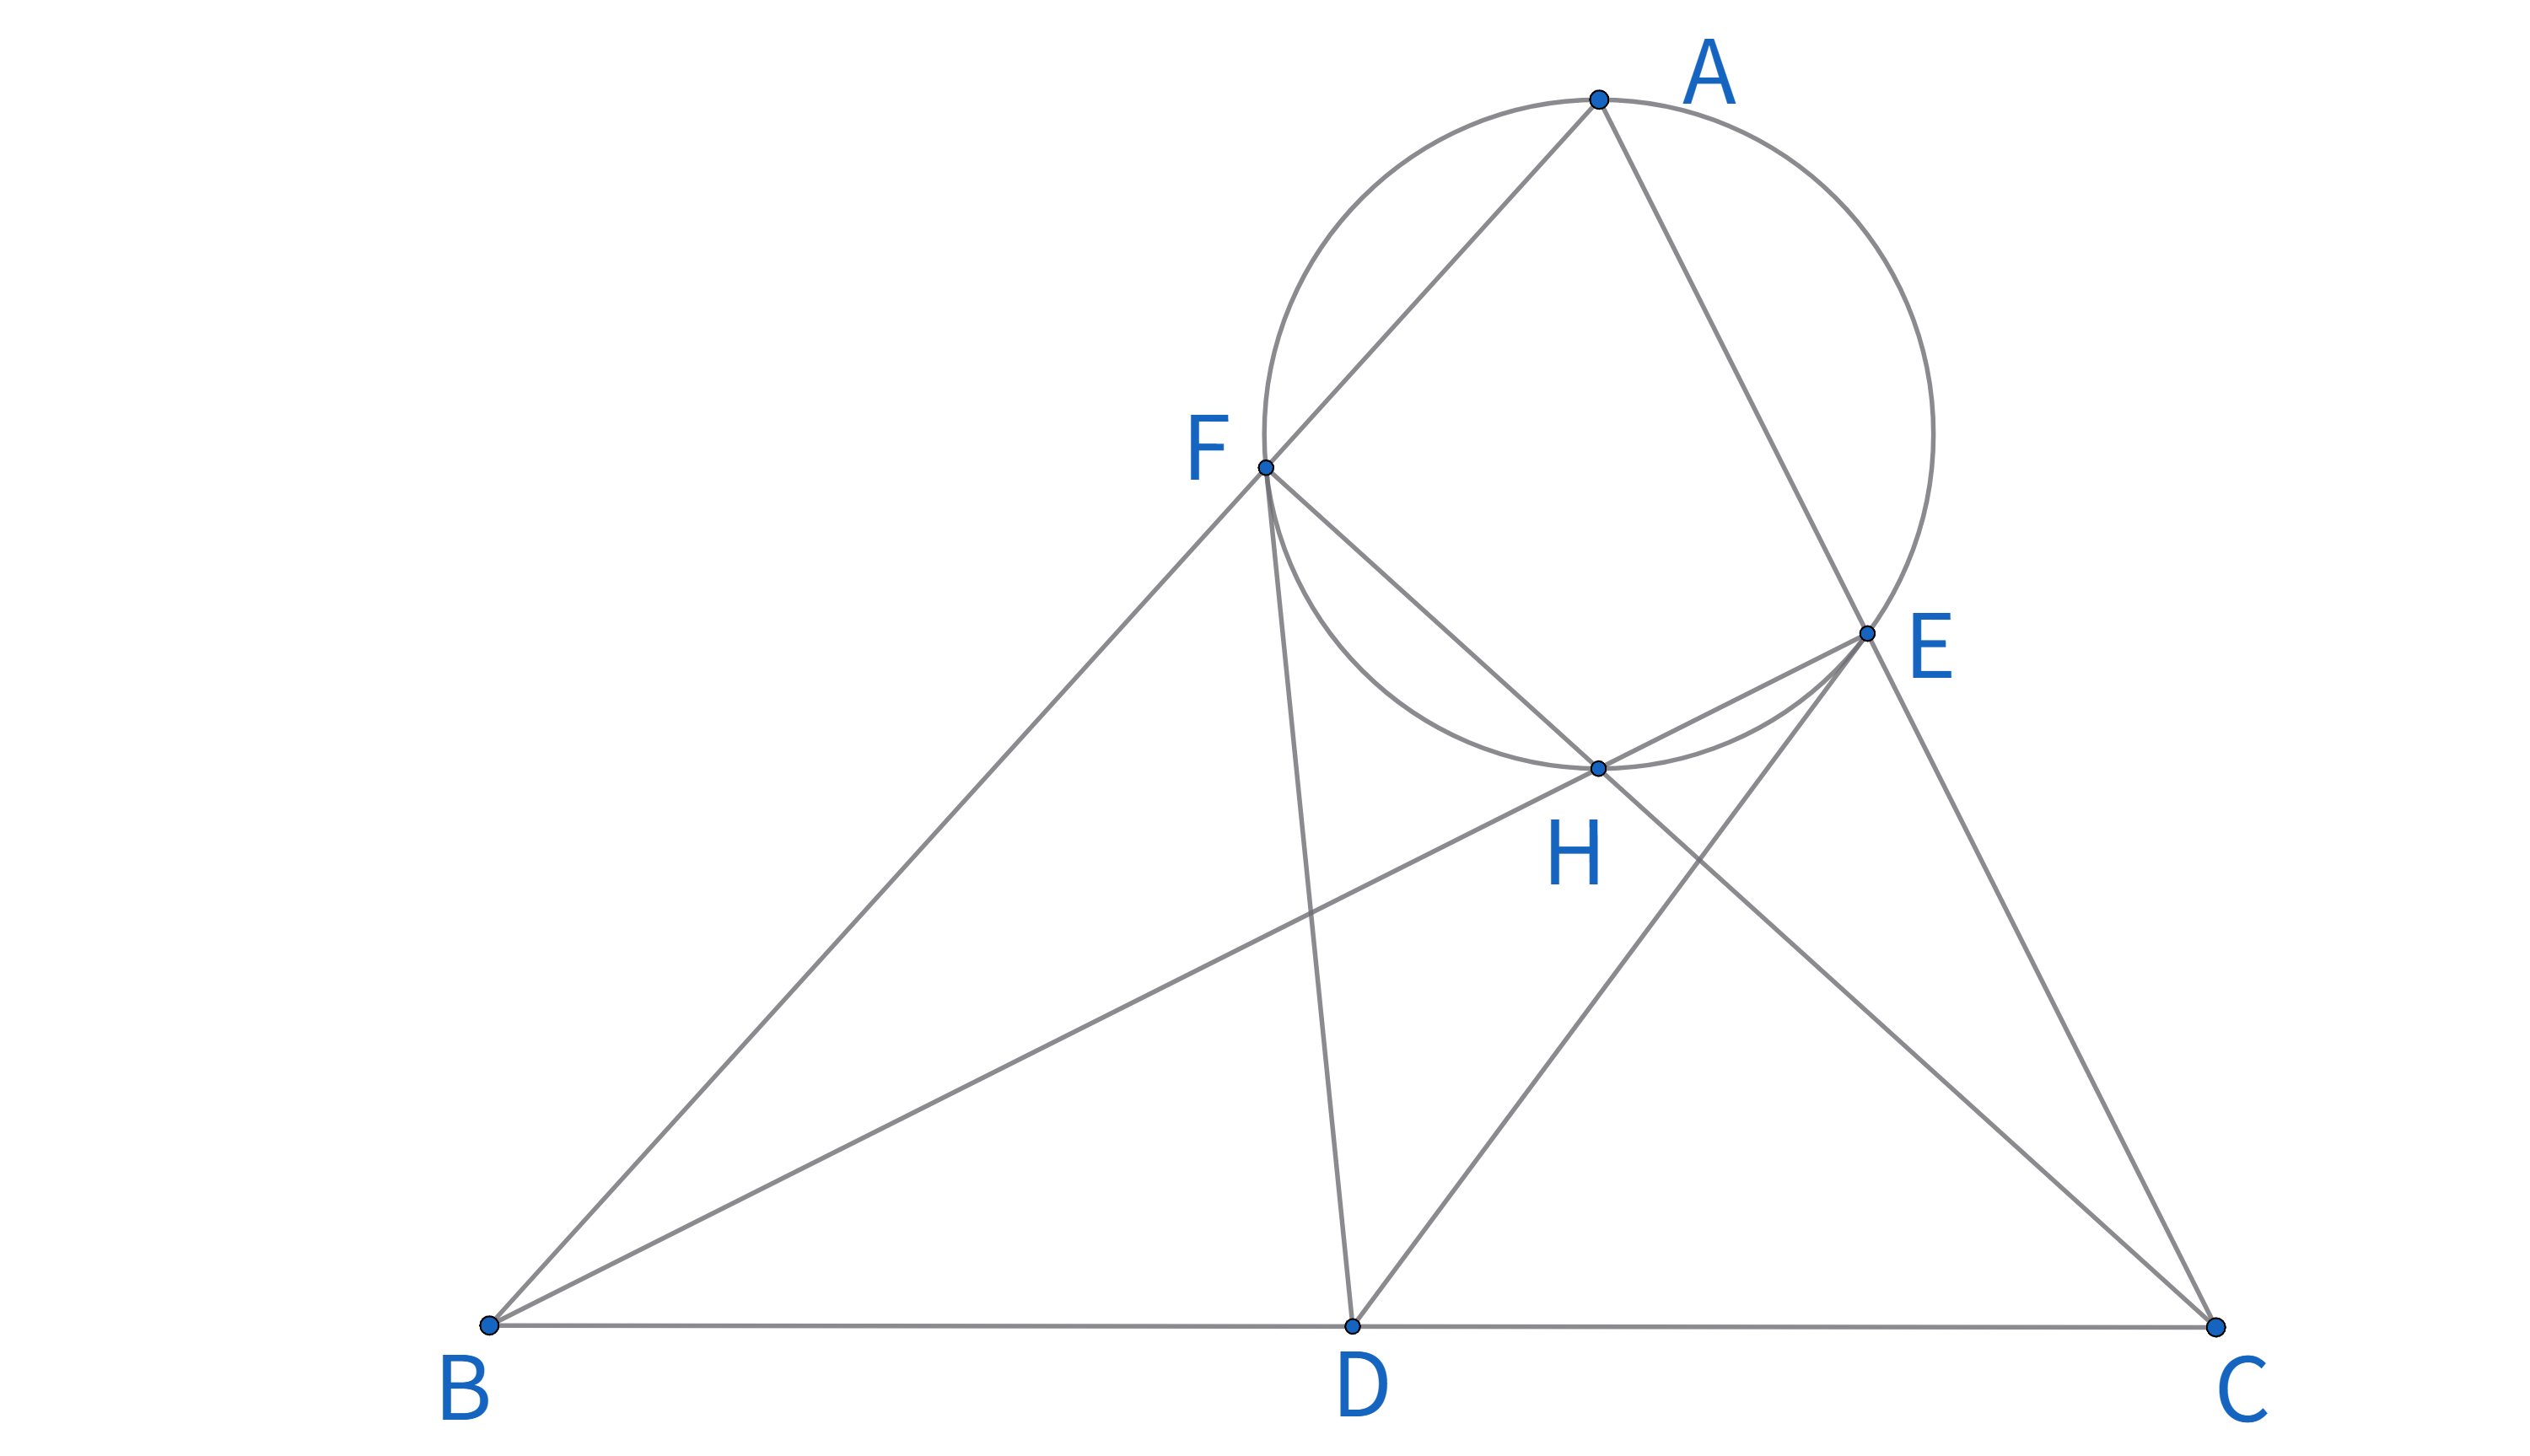
\includegraphics[width=0.7\linewidth]{figures/exercises/009.png}
\end{figure}


\begin{exercise}
(内切圆弦上的直线) 设 $\triangle ABC$ 的内切圆在边 $BC, {CA}, {AB}$ 上的切点分别是 $D, E, F$,内切圆圆心为 $I$。设 $M, N$ 分别是 $BC, AC$ 的中点。射线 $BI$ 与直线 $EF$ 相交于 $K$。证明:$BK \perp CK$,并且 $K$ 在直线 $MN$ 上。
\end{exercise}
\begin{figure}[H]
    \centering
    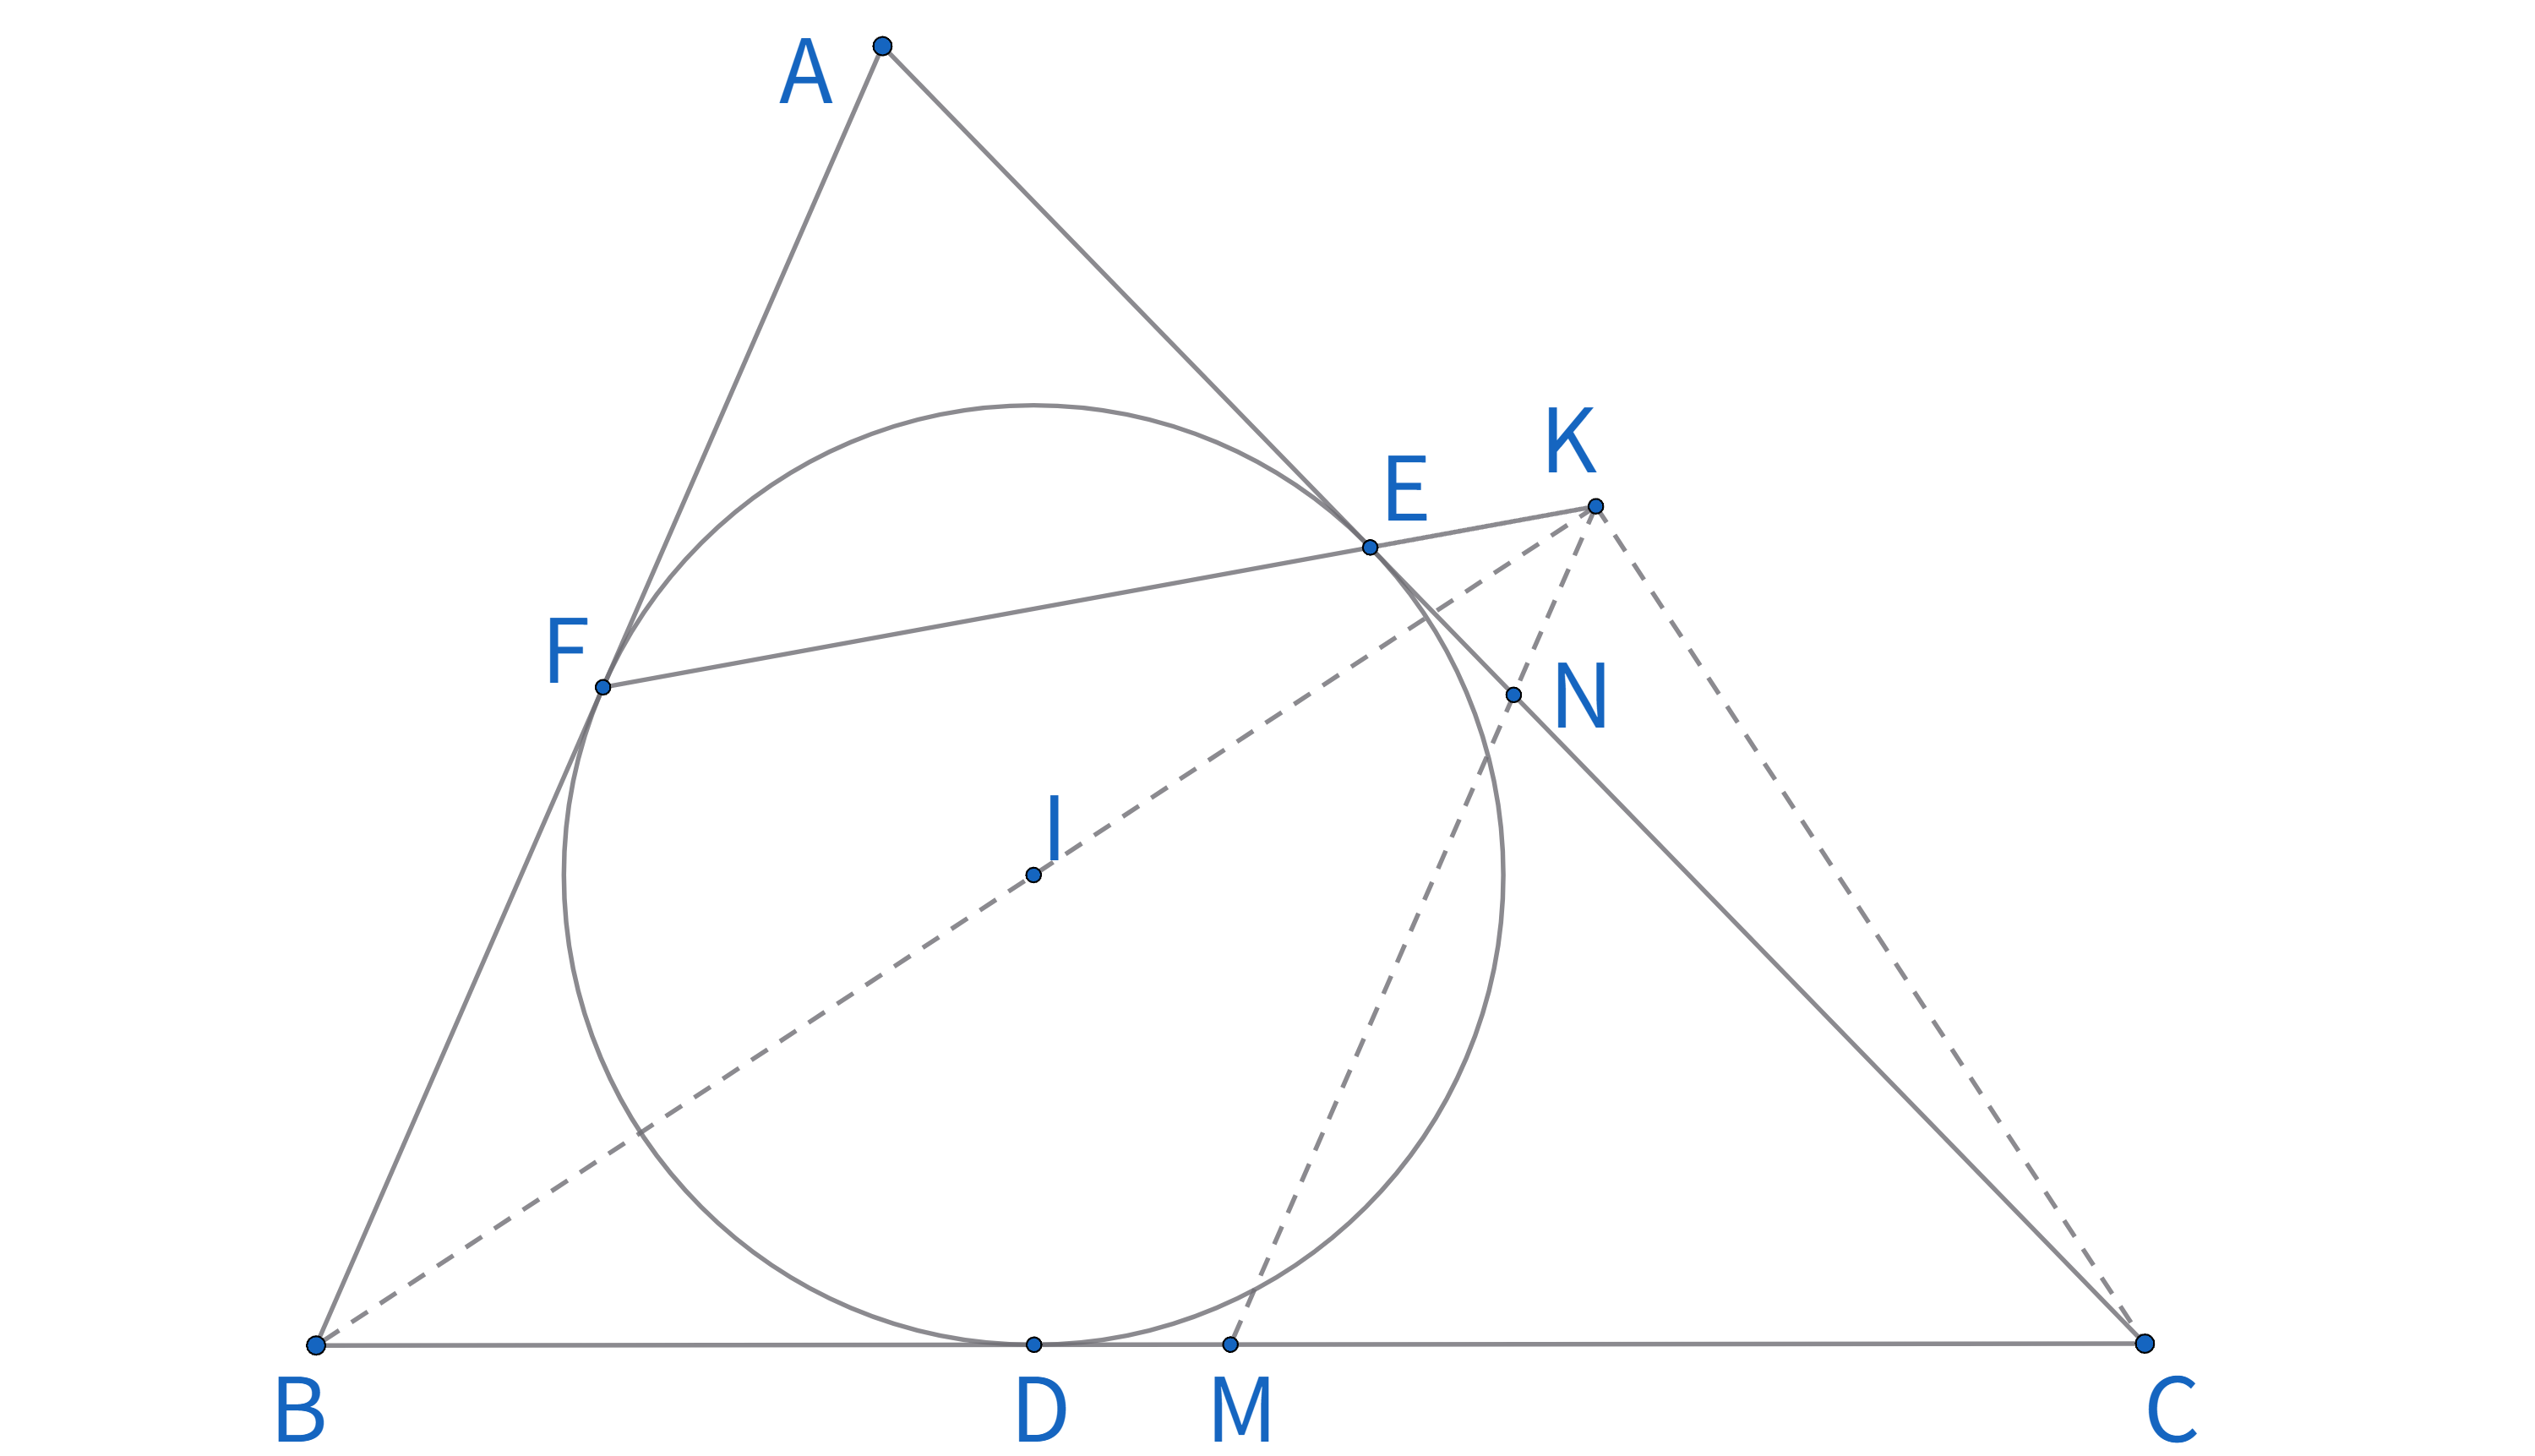
\includegraphics[width=0.7\linewidth]{figures/exercises/010.png}
\end{figure}

\newpage 
\begin{exercise}
(加拿大 1997/4) 点 $O$ 在平行四边形 $ABCD$ 的内部,使得 $\angle AOB + \angle COD = 180^\circ$。证明:$\angle OBC = \angle ODC$。
\end{exercise}
\begin{figure}[H]
    \centering
    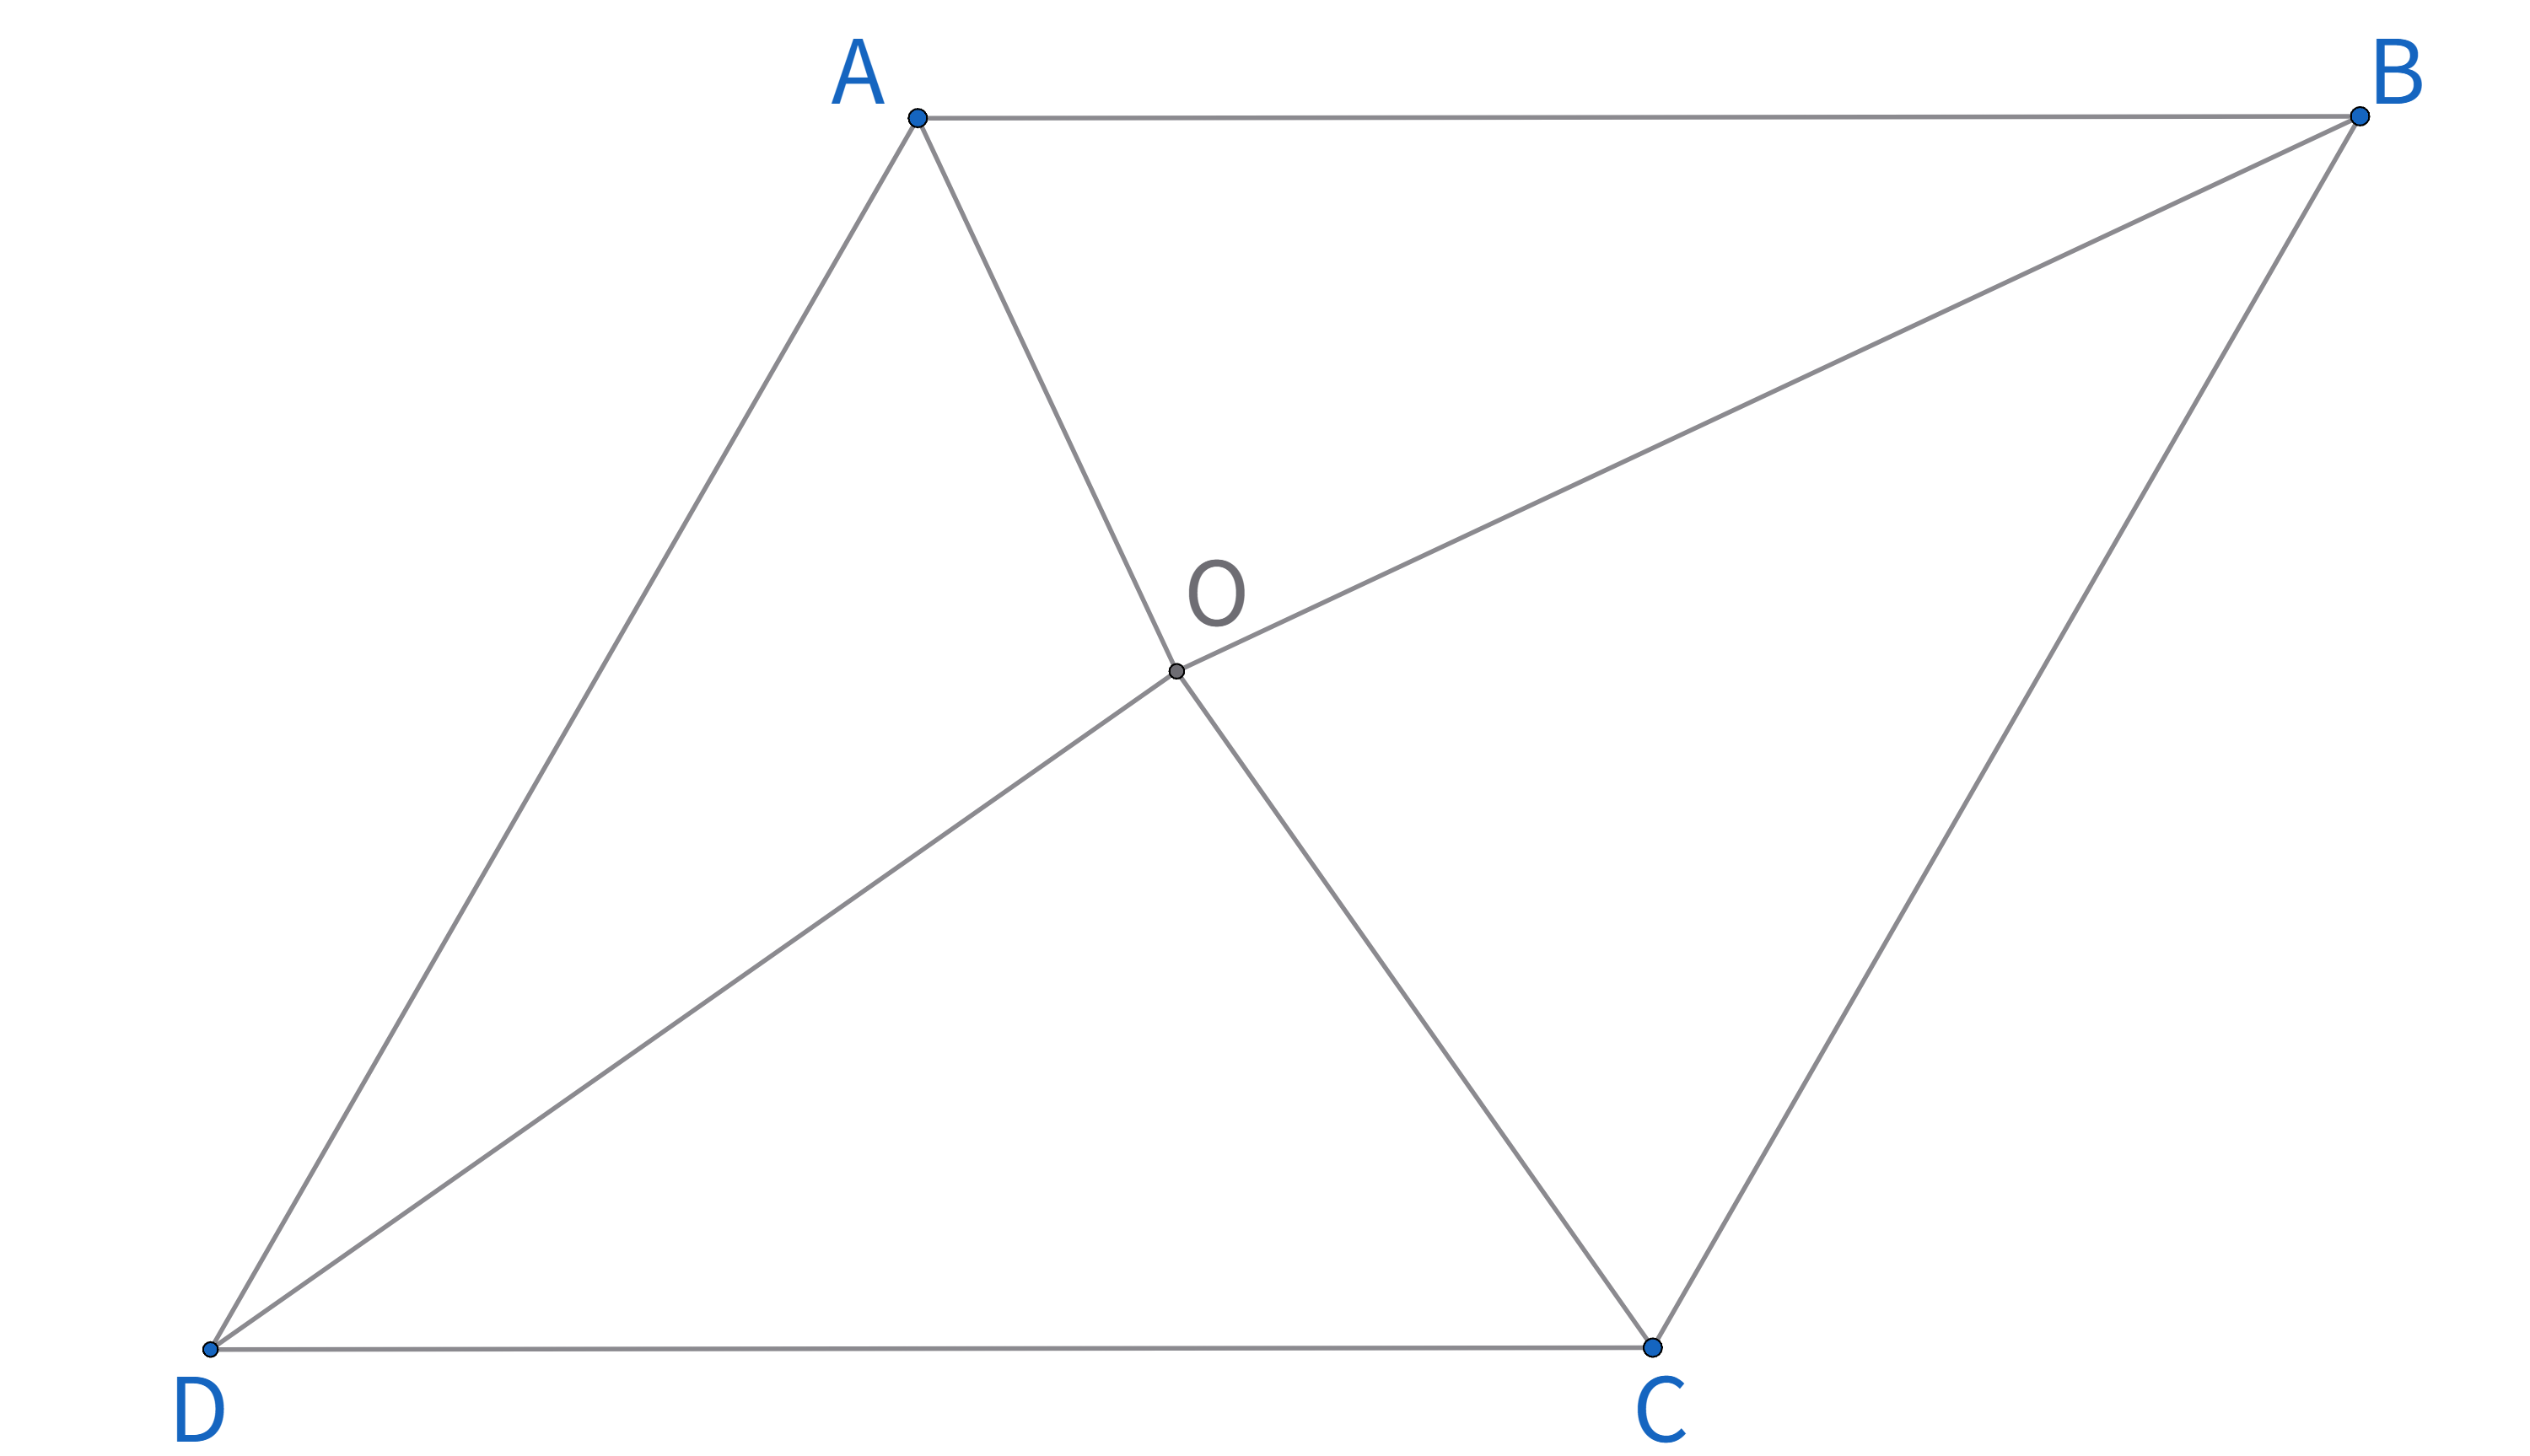
\includegraphics[width=0.7\linewidth]{figures/exercises/011.png}
\end{figure}


\begin{exercise}
(IMO 2006/1) 设 $\triangle ABC$ 的内心为 $I$,$P$ 在三角形内部,满足 $\angle PBA + \angle PCA = \angle PBC + \angle PCB$。证明:$AP \geq AI$,等号成立当且仅当 $P = I$。
\end{exercise}
\begin{figure}[H]
    \centering
    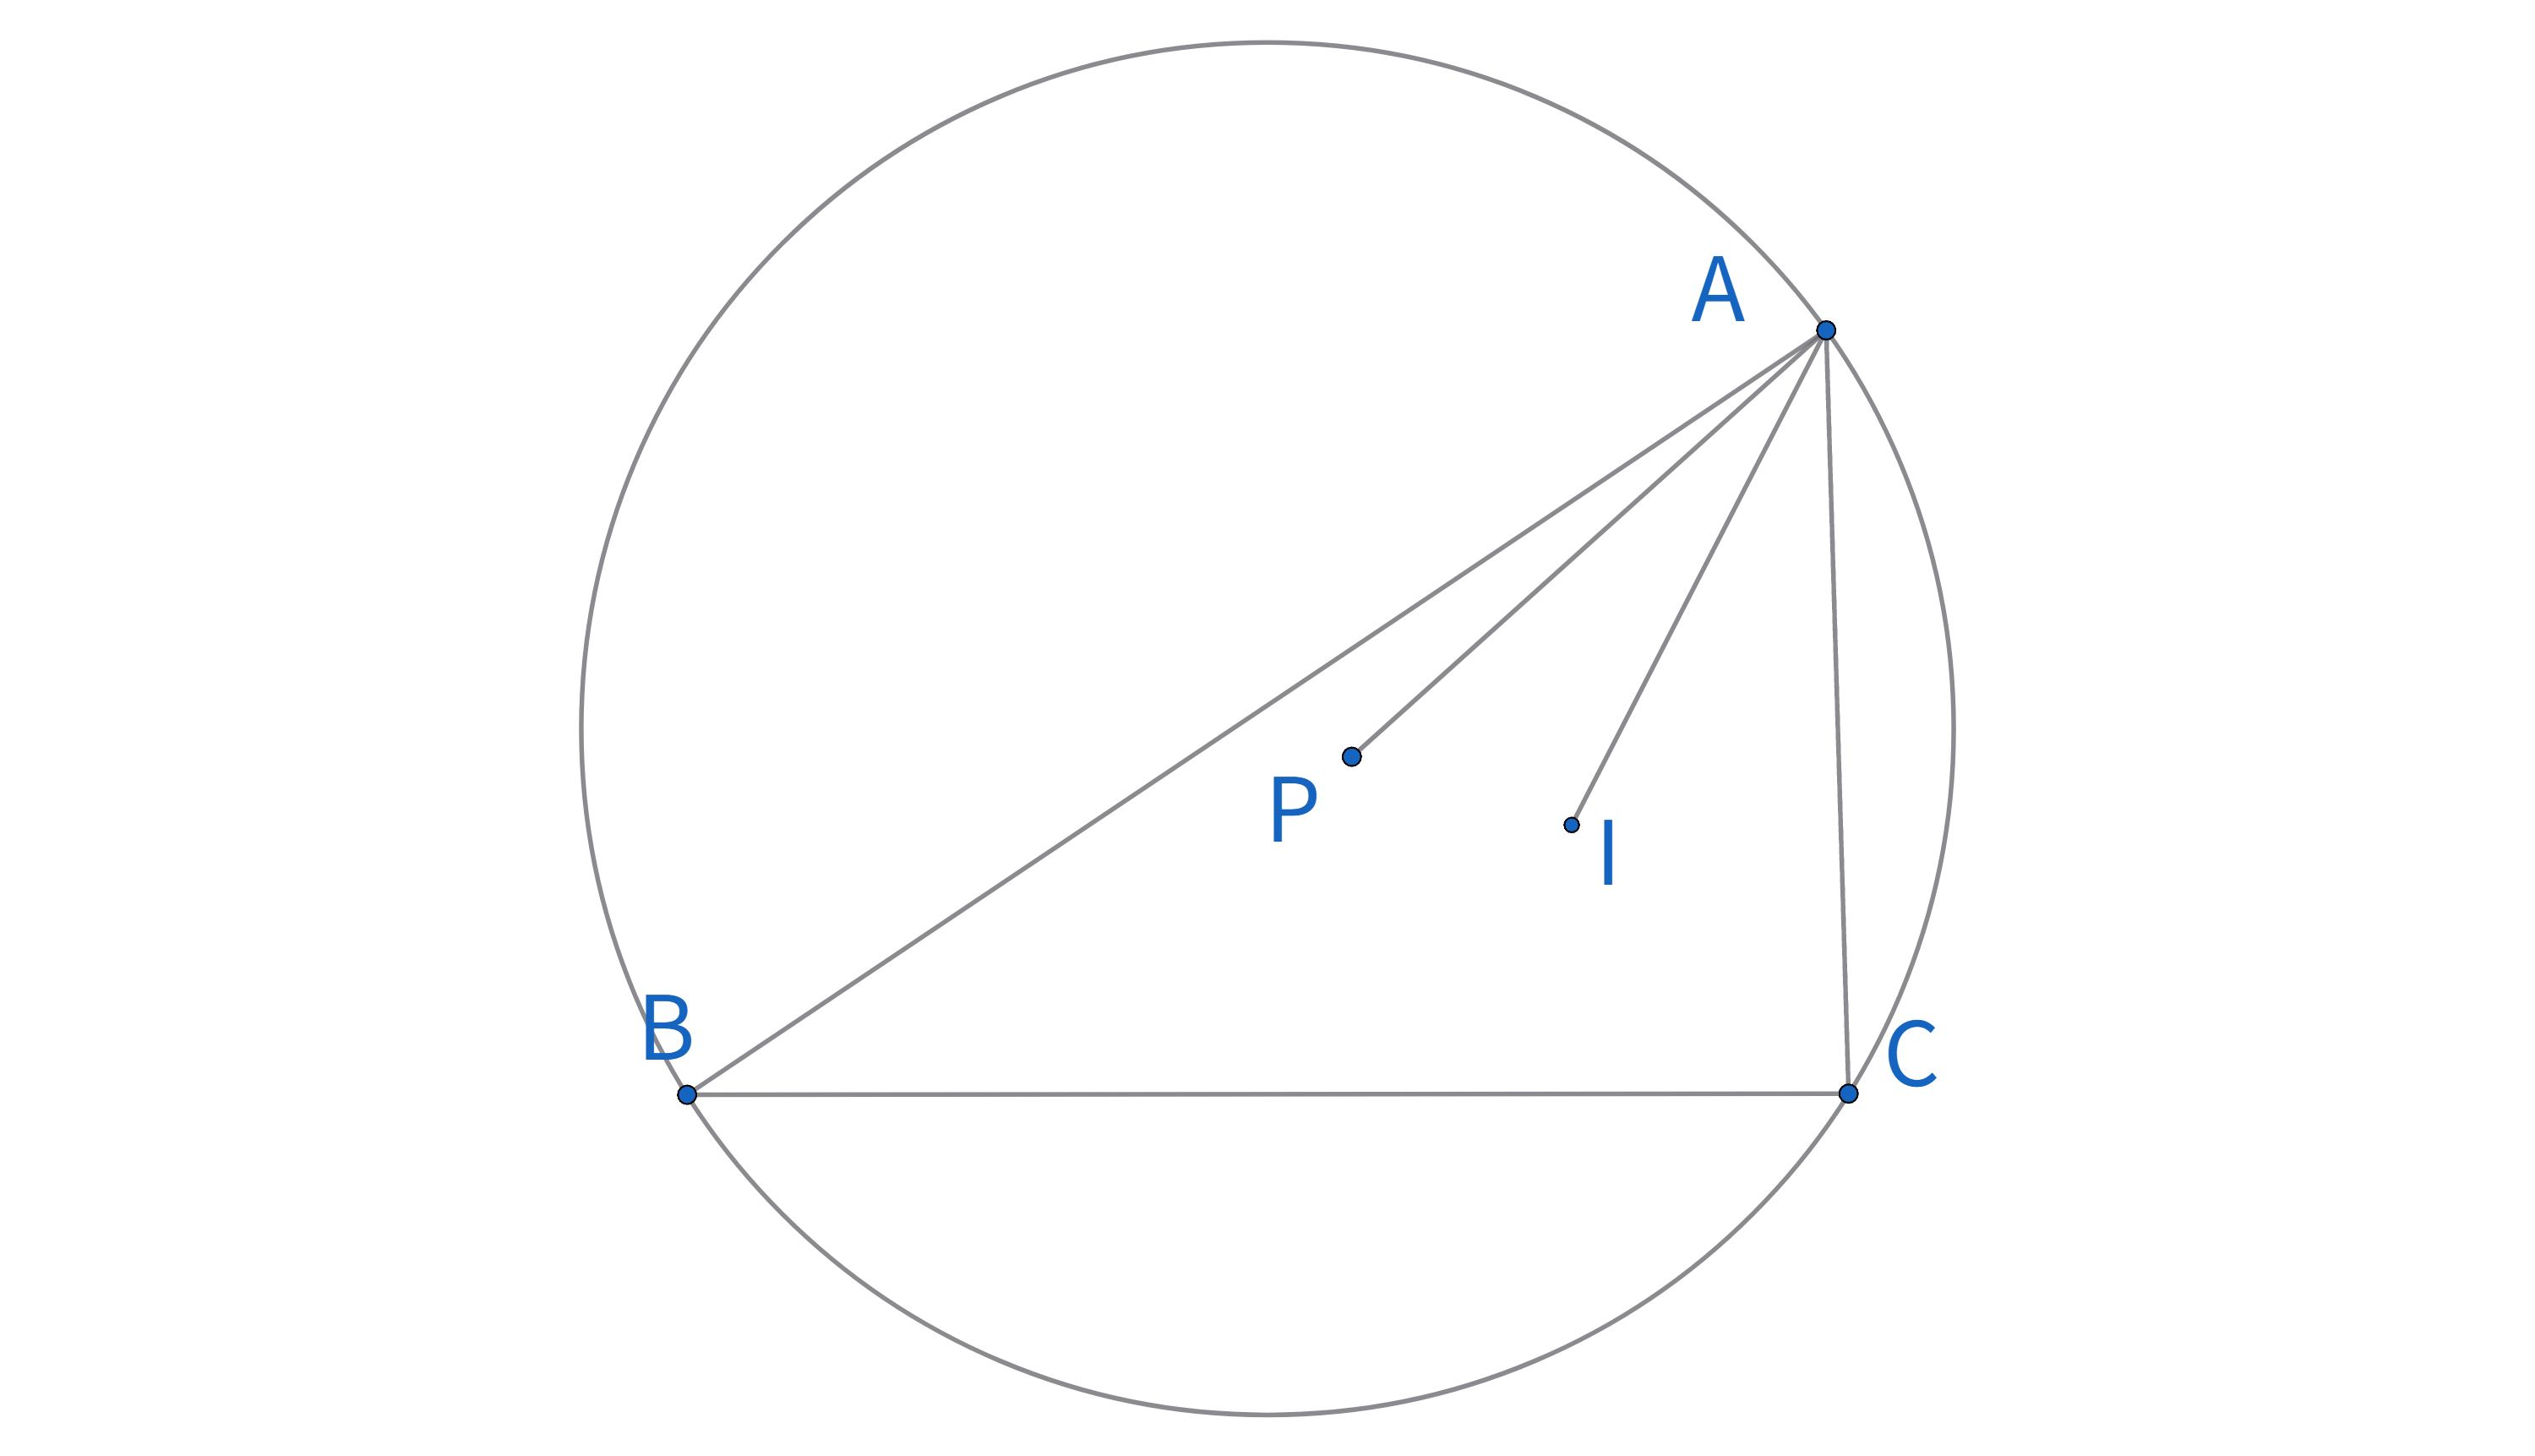
\includegraphics[width=0.7\linewidth]{figures/exercises/012.png}
\end{figure}


\newpage 
\begin{exercise}
(西姆松线) 如图1.8D,设 $P$ 是 $\triangle ABC$ 外接圆上任一点,$X, Y, Z$ 分别是从 $P$ 到直线 $BC, CA, AB$ 的投影。证明:$X, Y, Z$ 共线。
\end{exercise}
\begin{figure}[H]
    \centering
    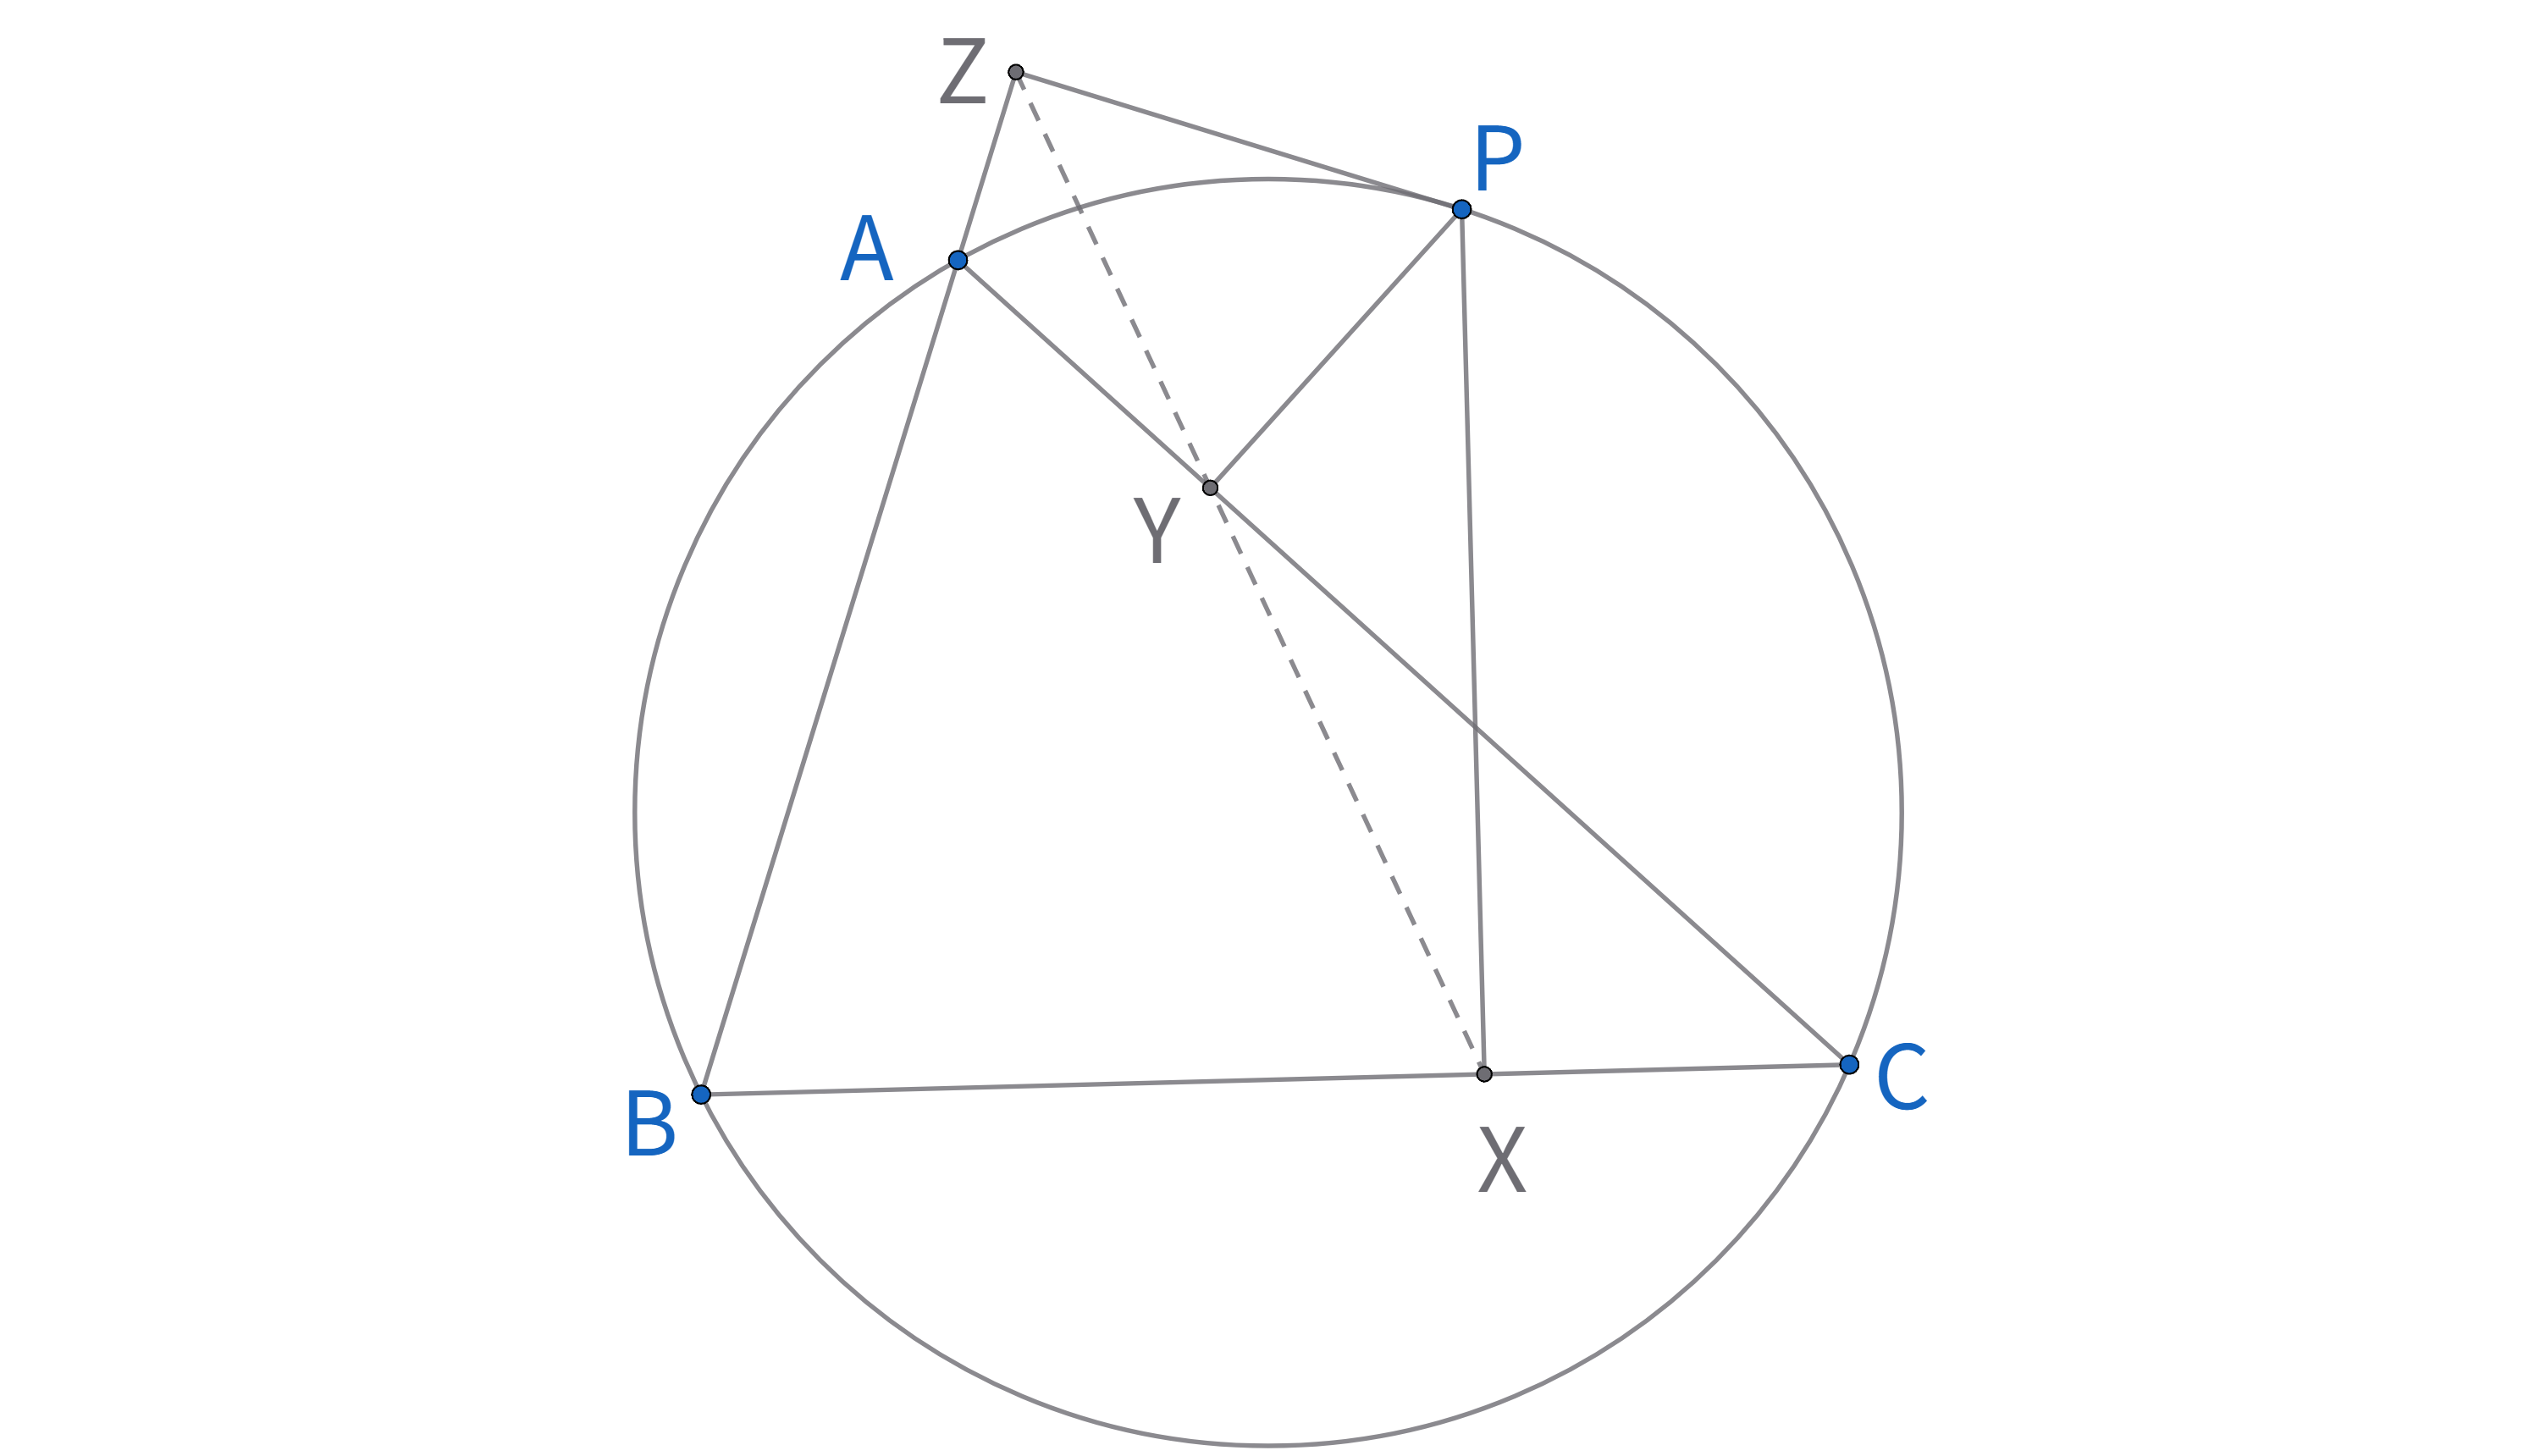
\includegraphics[width=0.7\linewidth]{figures/exercises/013.png}
\end{figure}

\begin{exercise}
(USAMO 2010/1) 设凸五边形 $AXYZB$ 内接于以 $AB$ 为直径的半圆。记 $P, Q, R, S$ 分别是 $Y$ 到直线 $AX, BX, AZ, BZ$ 上的投影。证明:直线 $PQ$ 和 $RS$ 形成的锐角是 $\angle XOZ$ 的一半,其中 $O$ 是线段 $AB$ 的中点。
\end{exercise}
\begin{figure}[H]
    \centering
    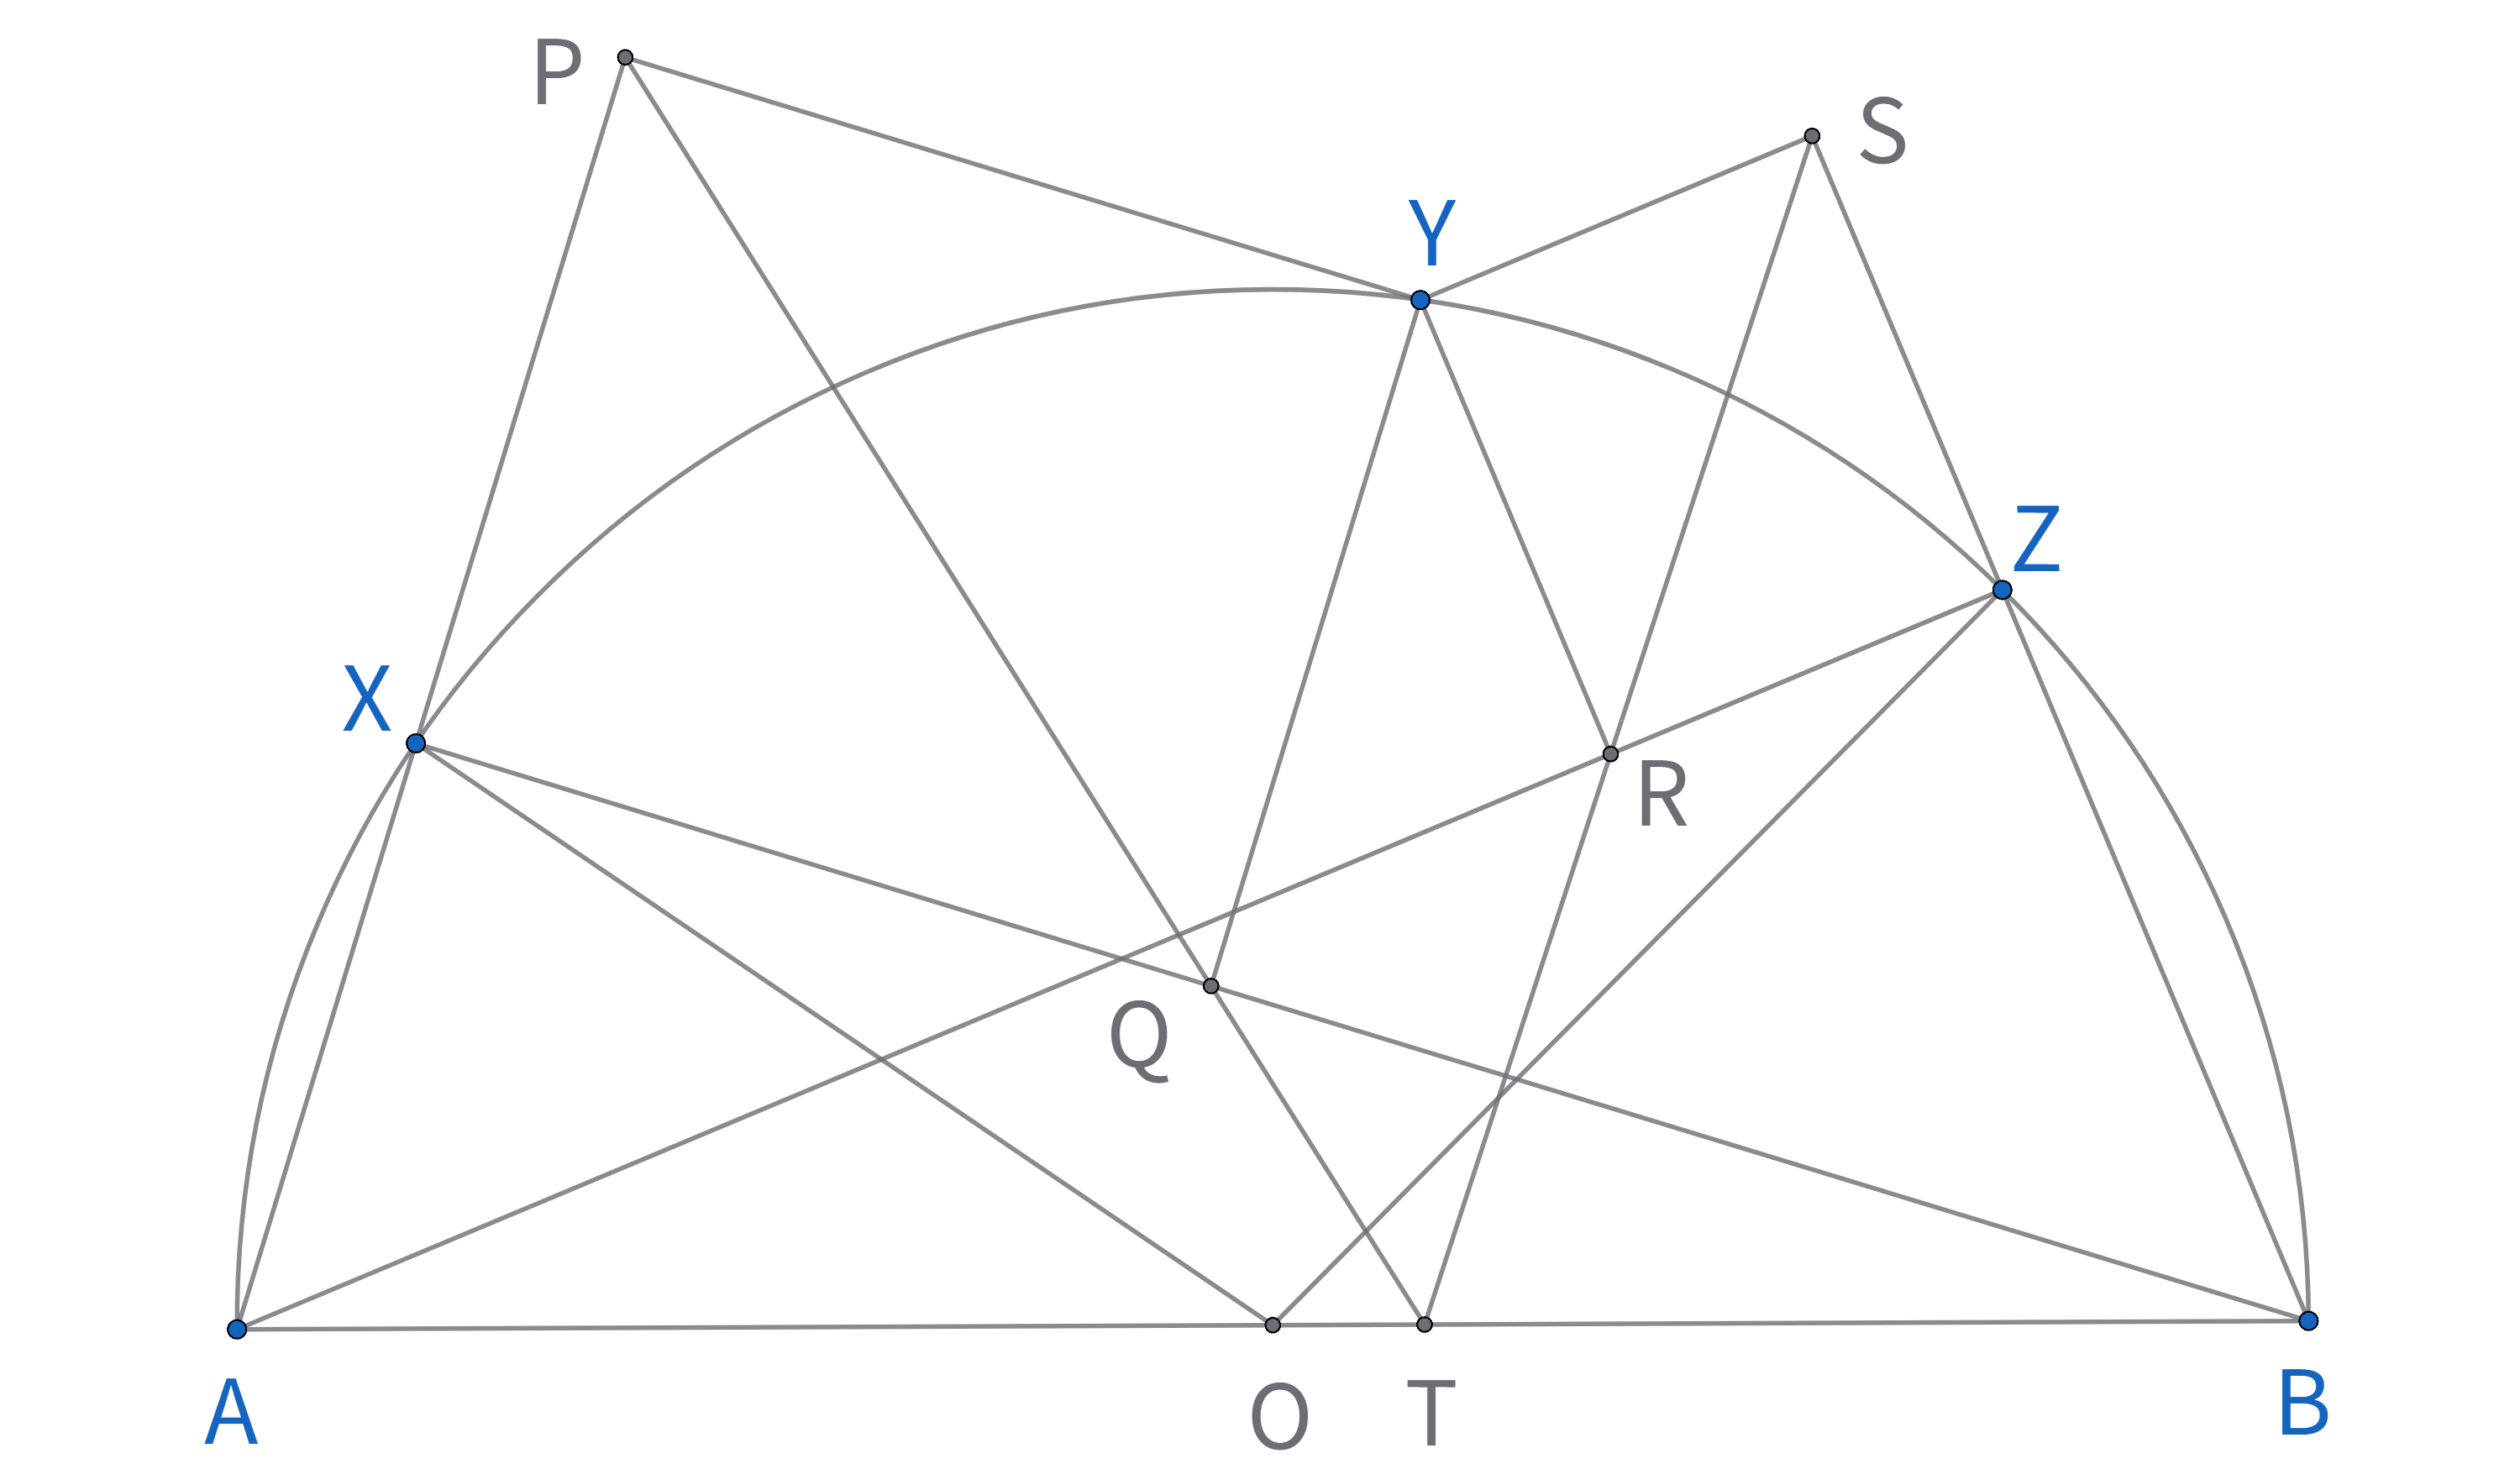
\includegraphics[width=0.7\linewidth]{figures/exercises/014.png}
\end{figure}


\newpage 
\begin{exercise}
(IMO 2013/4) 设锐角 $\triangle ABC$ 的垂心为 $H$,$W$ 是边 $BC$ 上一点,位于 $BC$ 中间。点 $M, N$ 分别是从 $B, C$ 引出的三角形的高的垂足。$\omega_1$ 是 $\triangle BWN$ 的外接圆,点 $X$ 满足 $WX$ 是 $\omega_1$ 的直径,类似地,点 $Y$ 满足 $WY$ 是 $\triangle CWM$ 外接圆 $\omega_2$ 的直径。证明:点 $X, Y, H$ 共线。(如果改为$\triangle BWM, \triangle CWN$的外接圆,结论变为X,Y,A共线。)
\end{exercise}
\begin{figure}[H]
    \centering
    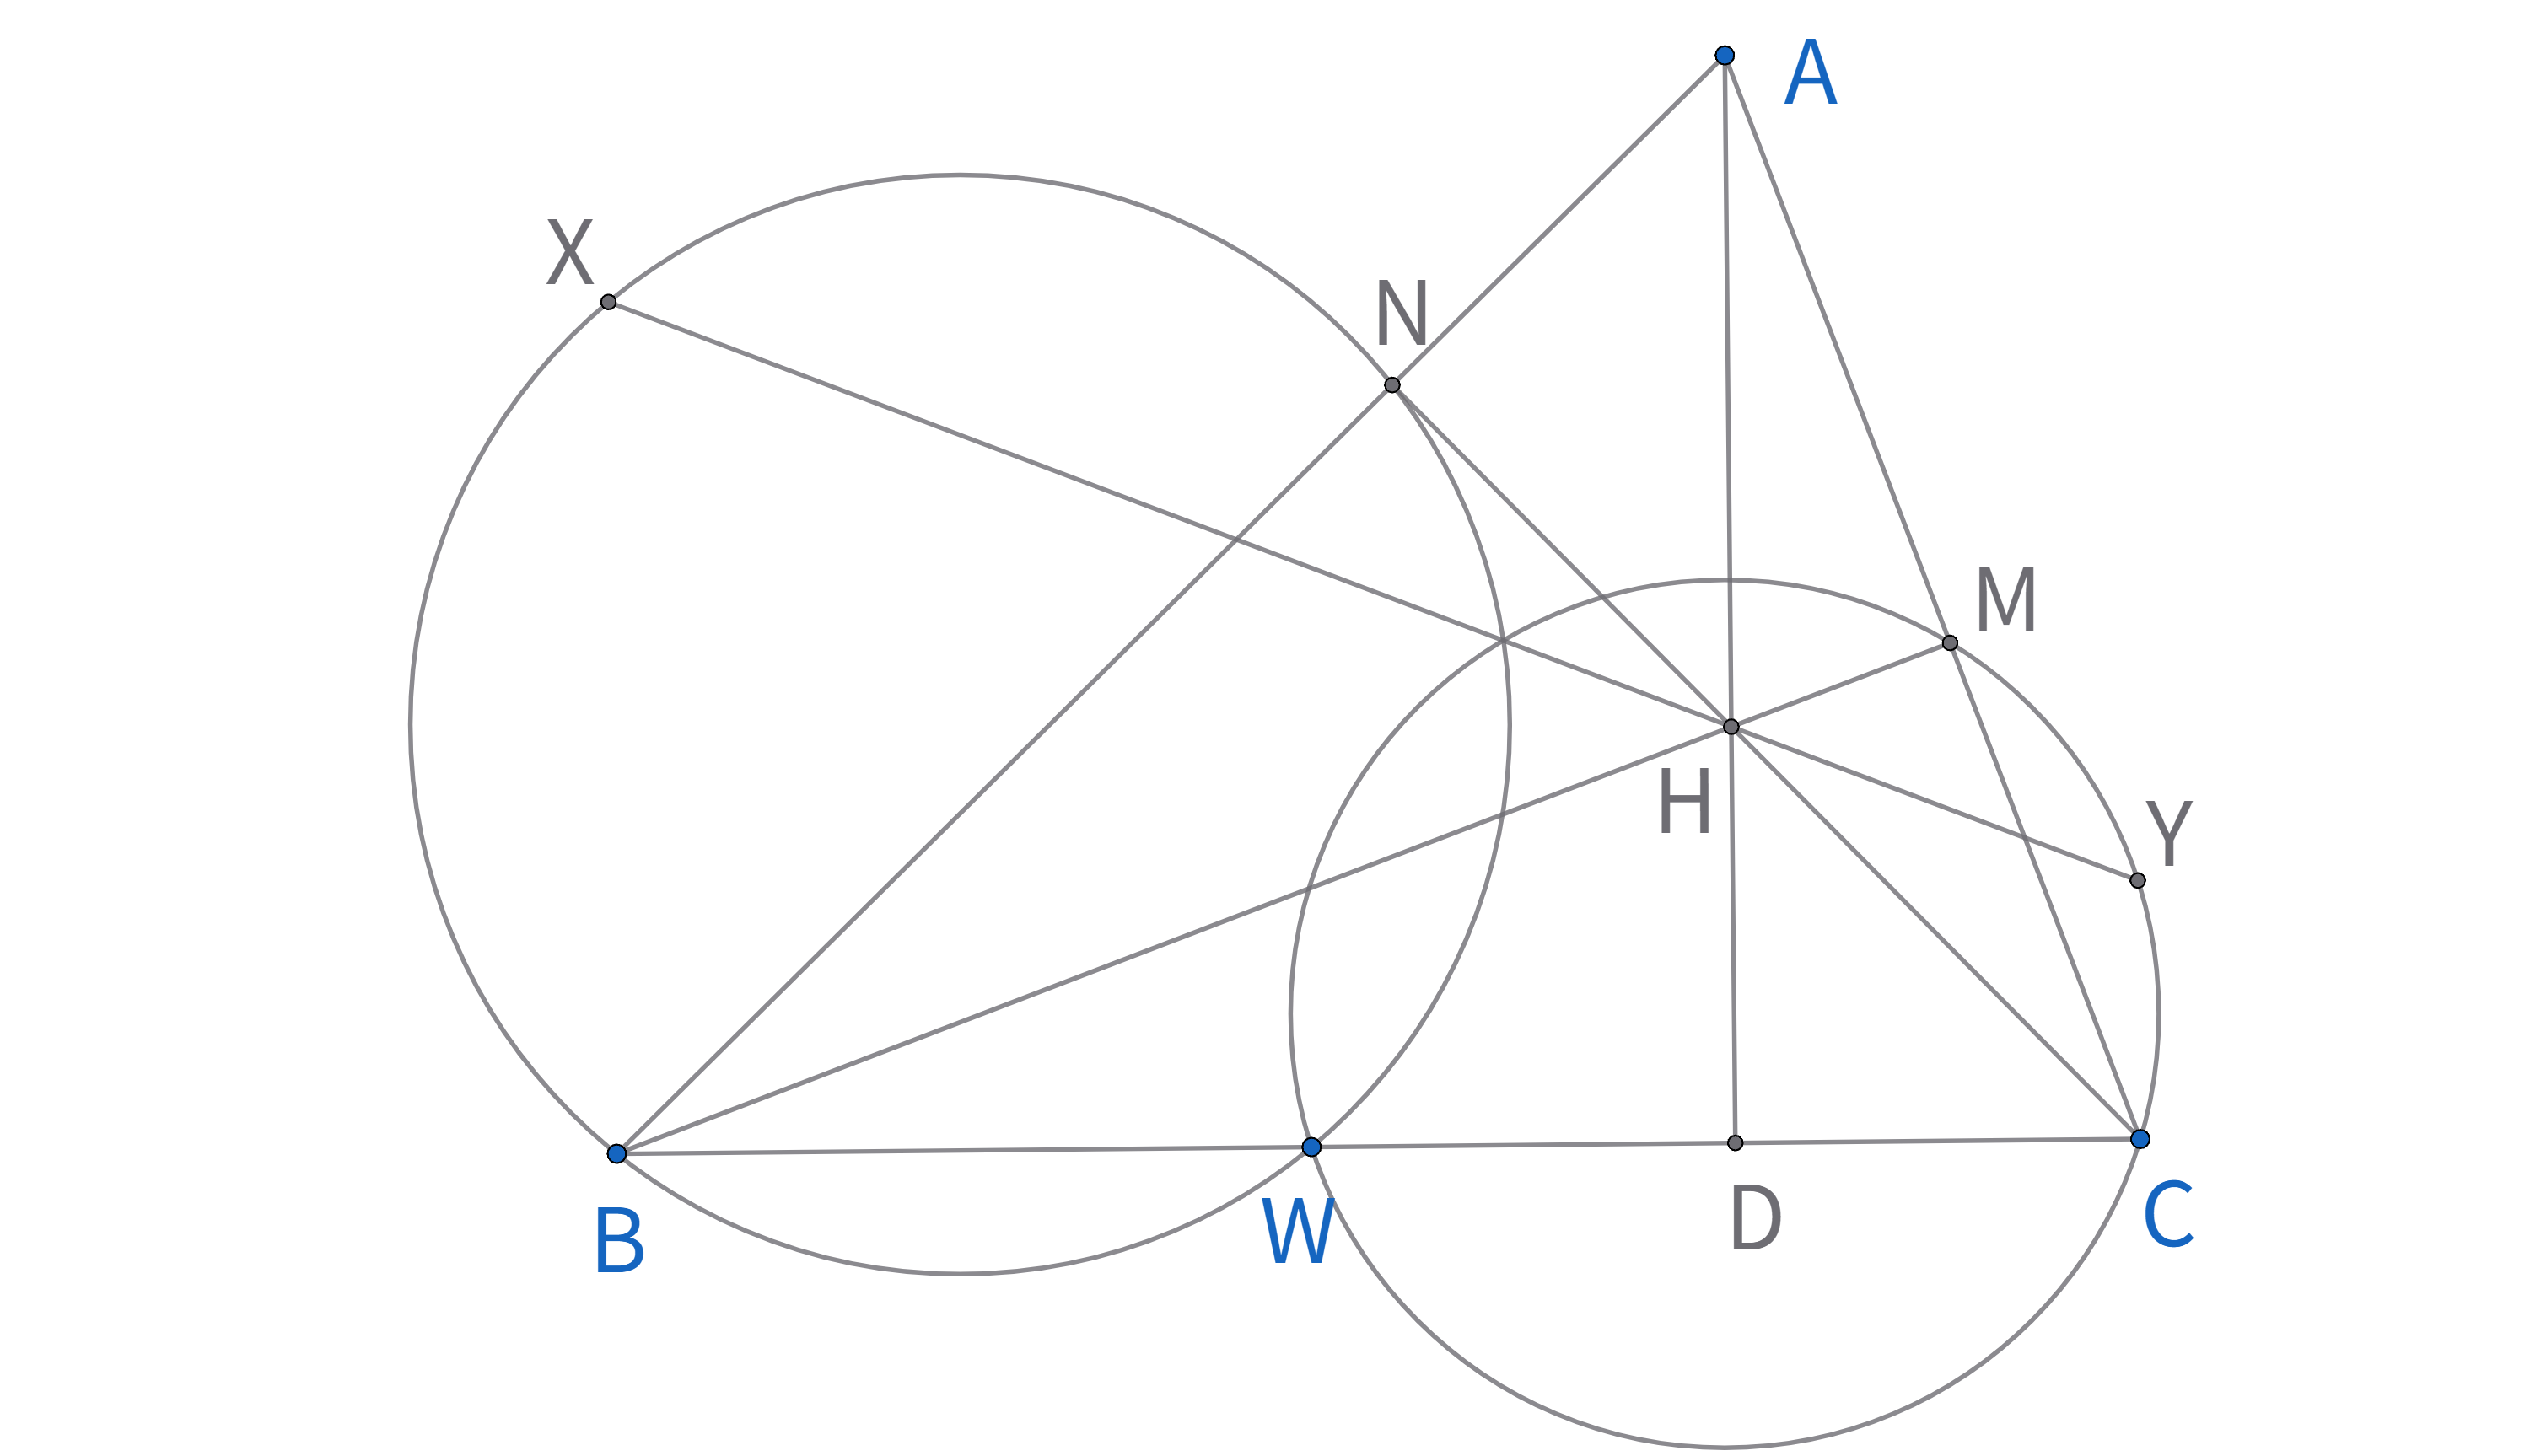
\includegraphics[width=0.7\linewidth]{figures/exercises/015.png}
\end{figure}


\begin{exercise}
(IMO 1985/1) 某个圆的圆心在圆内接四边形 $ABCD$ 的边 ${AB}$ 上,并且与另外三边相切。证明:$AD + BC = AB$。
\end{exercise}
\begin{figure}[H]
    \centering
    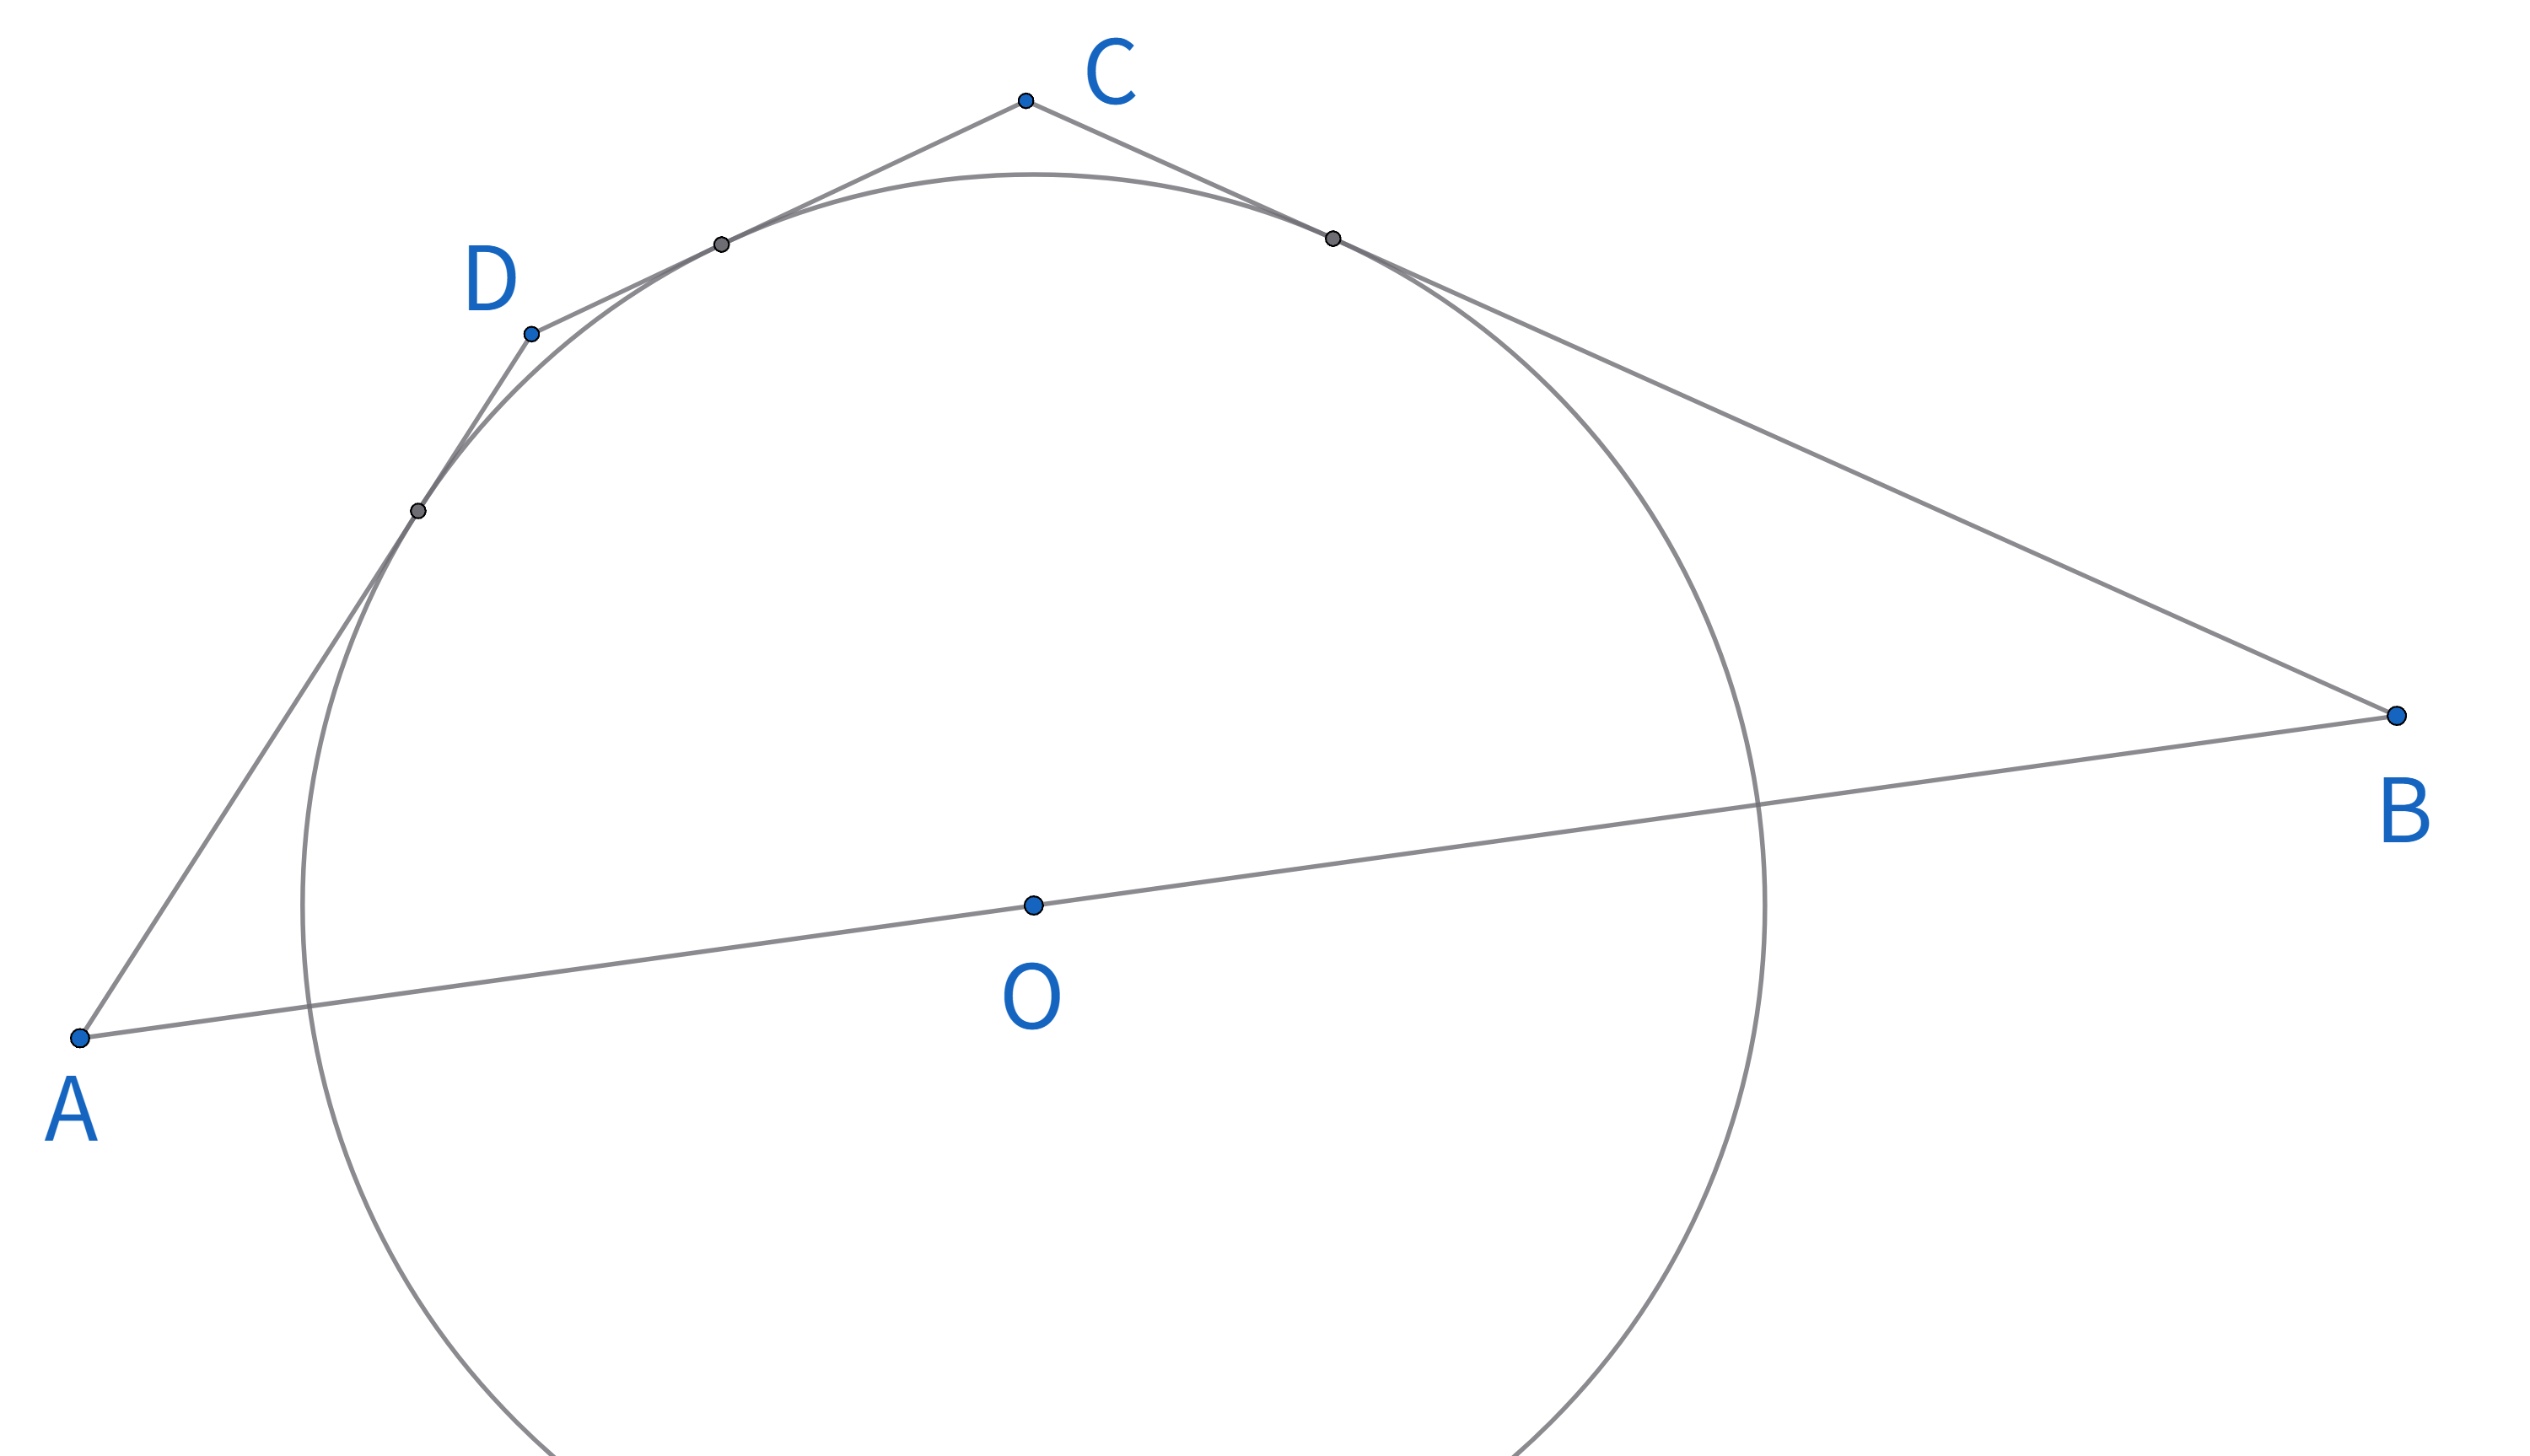
\includegraphics[width=0.7\linewidth]{figures/exercises/016.png}
\end{figure}


\newpage 

\begin{exercise}
在$\triangle ABC$中AB=AC,AD为中线,P为AD上的一点,过C做CF平行于AB,延长BP交AC于E交CF于F。求证:

$$BP^2=PE\cdot PF.$$
\end{exercise}
\begin{figure}[H]
    \centering
    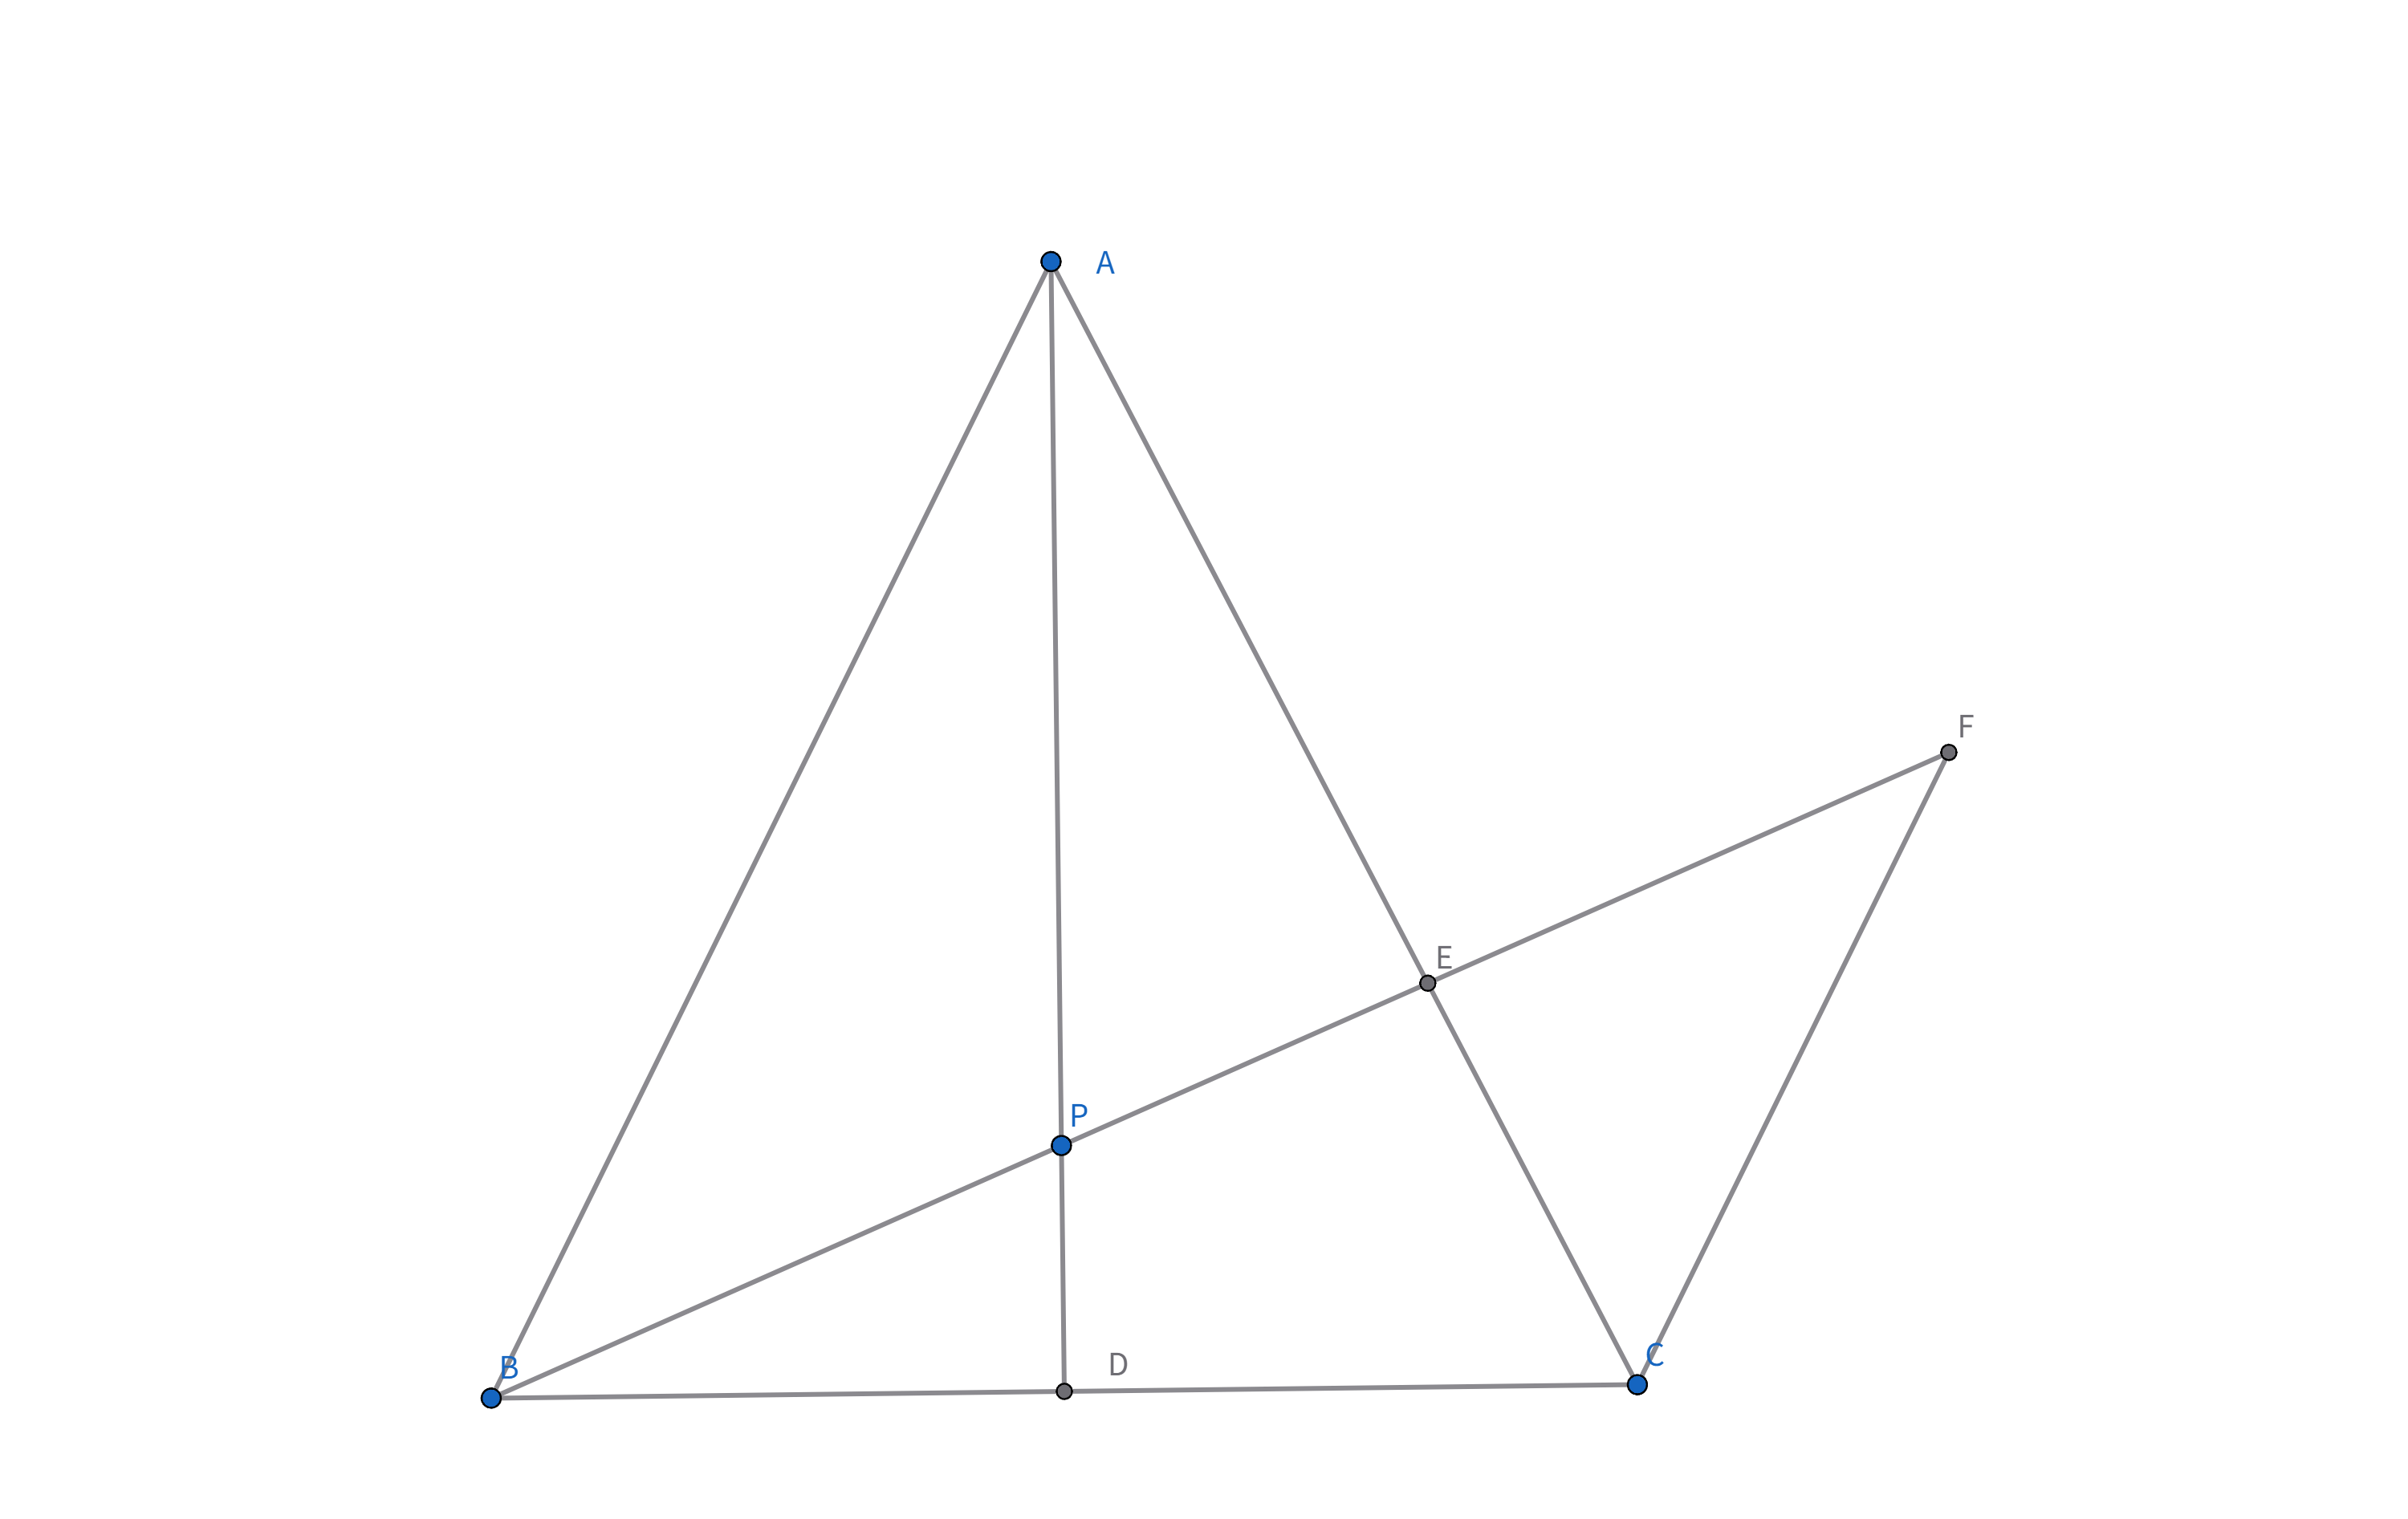
\includegraphics[width=0.7\linewidth]{figures/exercises/017.png}
\end{figure}


\begin{exercise}
不等边锐角$\triangle ABC$中,D为底边BC上一点,AD上有一点P,延长BP、CP,分别交AC、AB于M、N,若DA平分$\angle MDN$,证明$AD \perp BC.$
\end{exercise}
\begin{figure}[H]
    \centering
    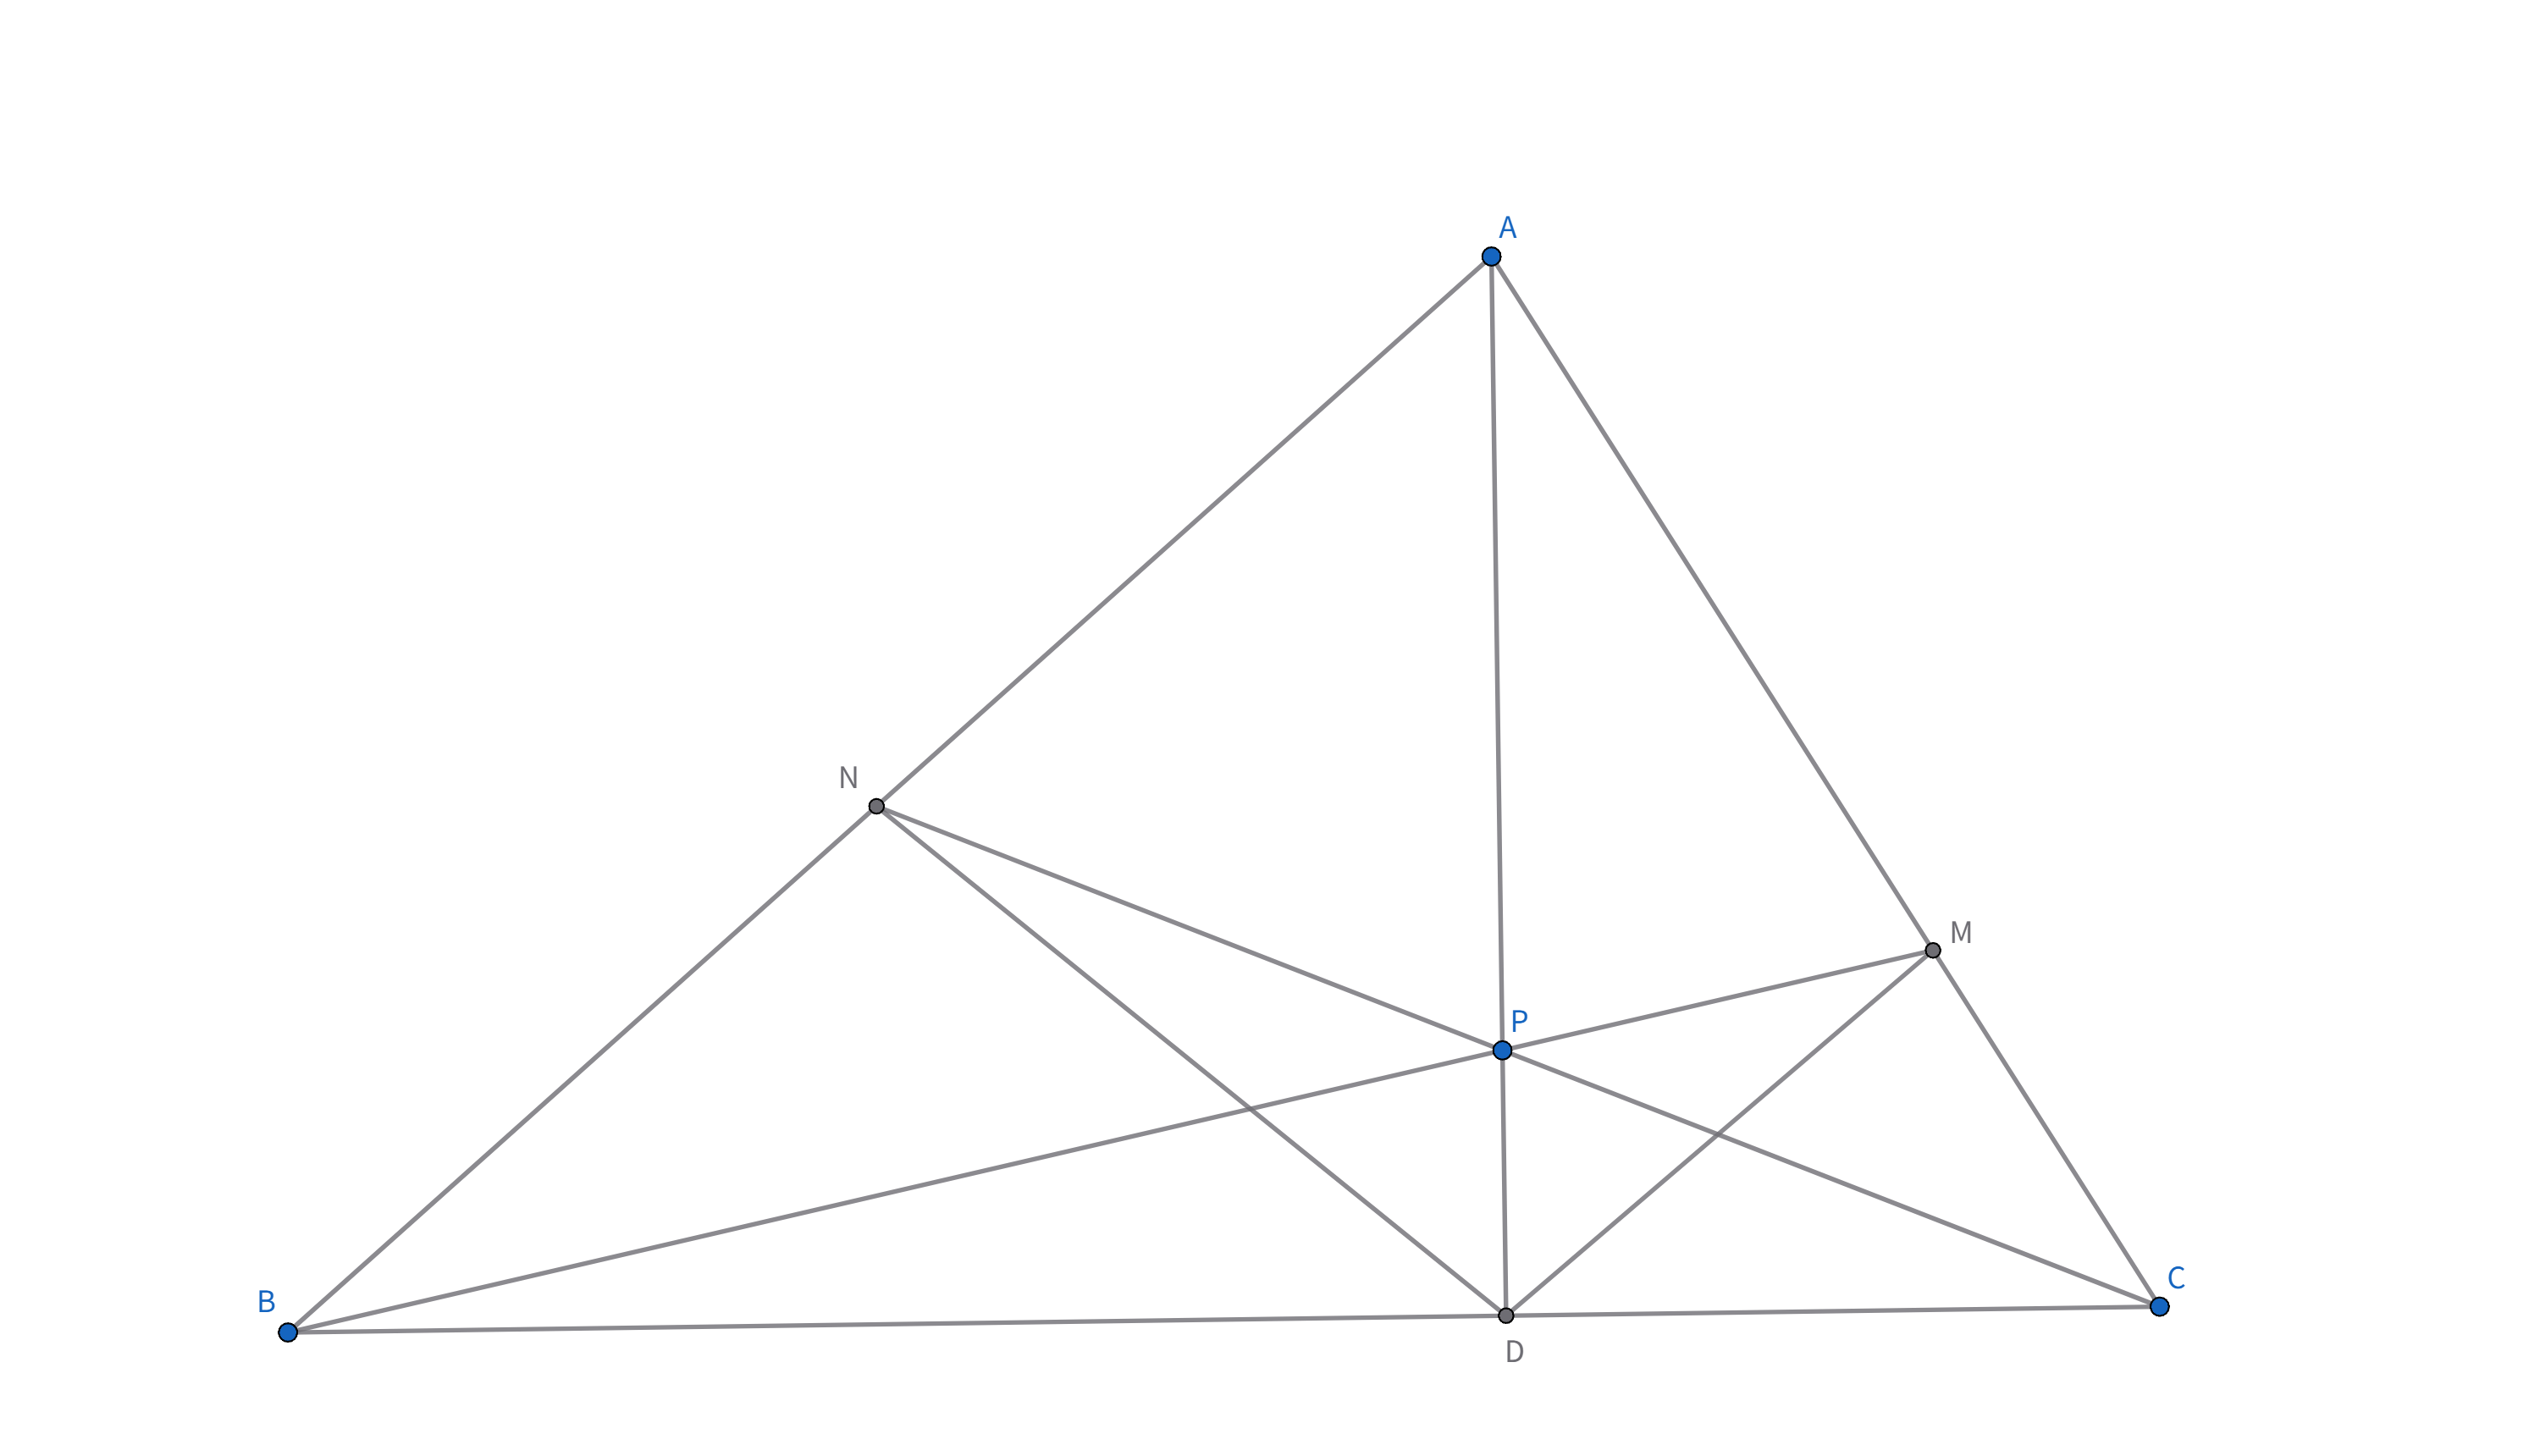
\includegraphics[width=0.7\linewidth]{figures/exercises/018.png}
\end{figure}    